\section{Measurement of Dijet Mass Spectrum}

In this section we explain how we measure the 
dijet mass spectrum in data, compare it with
the Monte Carlo predictions for QCD, and fit it
to a simple parameterization to test the smoothness 
of the data.

\subsection{Data Sample}

Our collision dataset was 
\begin{verbatim}
     (135059-135735) /MinimumBias/Commissioning10-SD_JetMETTau-Jun14thSkim_v1/RECO
     (136066-137028) /JetMETTau/Run2010A-Jun14thReReco_v2/RECO
     (137437-139558) /JetMETTau/Run2010A-PromptReco-v4/RECO
     (139779-140159) /JetMETTau/Run2010A-Jul16thReReco-v1/RECO
     (140160-141899) /JetMETTau/Run2010A-PromptReco-v4/RECO
     (141900-144114) /JetMET/Run2010A-PromptReco-v4/RECO 
\end{verbatim}
The reconstruction software (CMSSW\_3\_6\_1\_patch4) and conditions are identical for all three datasets listed above.
We run over this dataset at the Fermilab LPC and select the runs taken during
April-August 2010:
\begin{verbatim}

135149, 135175, 135521, 135523, 135525, 135528, 135535, 135575, 135735,
136066, 136082, 136087, 136088, 136097, 136100, 136119, 137027, 137028,
138572, 138737, 138738, 138739, 138742, 138744, 138745, 138746, 138747,
138750, 138751, 138919, 138920, 138921, 138923, 138924, 138937, 138939, 
139020, 139096, 139098, 139100, 139102, 139103, 139195, 139239, 139347, 
139356, 139360, 139364, 139365, 139368, 139370, 139372, 139375, 139399, 
139400, 139407, 139411, 139457, 139458, 139459, 139779, 139780, 139781, 
139784, 139786, 139788, 139789, 139790, 139965, 139966, 139967, 139968, 
139969, 139971, 139972, 139973, 139974, 139975, 140058, 140059, 140070, 
140076, 140119, 140123, 140124, 140126, 140158, 140159, 140160, 140180, 
140181, 140331, 140359, 140361, 140362, 140379, 140381, 140382, 140383, 
140385, 140386, 140387, 140388, 140399, 140401, 141956, 141957, 141958, 
141959, 141960, 141961, 142035, 142036, 142038, 142039, 142040, 142076, 
142128, 142129, 142130, 142132, 142135, 142136, 142137, 142187, 142189, 
142191, 142264, 142265, 142303, 142304, 142305, 142308, 142309, 142311, 
142312, 142313, 142413, 142414, 142417, 142418, 142419, 142422, 142513, 
142514, 142523, 142524, 142525, 142528, 142530, 142535, 142537, 142557, 
142558, 142657, 142658, 142659, 142660, 142661, 142662, 142663, 142664, 
142928, 142933, 142935, 142936, 142953, 142954, 142970, 142971, 143004, 
143005, 143006, 143007, 143008, 143179, 143181, 143187, 143191, 143192, 
143193, 143318, 143319, 143320, 143321, 143322, 143326, 143327, 143328, 
143657, 143665, 143727, 143731, 143827, 143833, 143835, 143953, 143954, 
143955, 143956, 143957, 143959, 143960, 143961, 143962, 144011, 144086, 
144089, 144112, 144114
\end{verbatim}
The good run and luminosity section (LS) selection is based on the official CMS JSON files:
\begin{verbatim}
     Cert_135059-135735_7TeV_June14thReReco_Collisions10_JSON.txt
     Cert_136066-137028_7TeV_June14thReReco_Collisions10_JSON.txt
     Cert_137437-139558_7TeV_StreamExpress_Collisions10_JSON.txt
     Cert_139779-140159_7TeV_July16thReReco_Collisions10_JSON.txt
     Cert_140160-141899_7TeV_StreamExpress_Collisions10_JSON.txt
     Cert_141900-144114_7TeV_StreamExpress_Collisions10_JSON.txt
\end{verbatim}
The integrated luminosity of the selected sample is estimated to be $2.875\,pb^{-1}$. 

The integrated luminosity is measured~\cite{PAS_EWK_10-004} using
signals from the Forward Hadronic Calorimeter. Two methods for
extracting a real-time relative instantaneous luminosity are used, with
absolute calibration using separation scans first pioneered by Van Der
Meer at the ISR~\cite{ref:VdM}. The systematic uncertainties corresponding to the
normalization constant is about 11\%.

We make the Technical Trigger bit TT0 selection for this sample which selects events consistent with the LHC bunch crossing.
Further we require that  each event has a good primary vertex with $z$ value within
15 cms of the center of the detector and a number of degrees of freedom of
at least 4. Finally, we only keep events that have at least one jet with raw $p_T>4$ GeV. This preselection job writes out root 
trees from the InclusiveJetTreeProducer on cmslpc.fnal.gov. 

\subsection{MC Samples}

\subsubsection{QCD}
For the comparison between data and simulation, we use the QCD Pythia MC where the phase space is
divided into 20 exclusive bins, based on the transverse momentum of the hard scattered parton ($\hat{p}_T$).
The MC samples used are:
\begin{verbatim}
/QCDDiJet_PtXXtoYY/Spring10-START3X_V26_S09-v1/GEN-SIM-RECO
\end{verbatim}
where XX and YY stand for the $\hat{p}_T$ boundaries. For the final comparison with the data, the MC samples
are weighted according to the cross-section and the number of events that were used.

\subsubsection{Resonances}
For resonance shapes we use the PYTHIA MC for excited quarks (Qstar) and Randall Sundrum 
Gravitons (RSGraviton) as discussed in the next section.  The samples used were
\begin{verbatim}
/RESONANCE_DiJetXX/Spring10-START3X_V26_S09-v1/GEN-SIM-RECO
/RESONANCEToJJ_M-YY_7TeV-pythia6/Spring10-START3X_V26-v1/GEN-SIM-RECO
\end{verbatim}
where RESONANCE is either "Qstar" or "RSGraviton",  XX is 700, 1200, or 2000 and YY is 500 or 3500, for those
masses in GeV.


\subsection{Software}
The analysis was done using the 
$CMSSW\_3\_6\_1$ release and the software is available in the CMS cvs system, through the following
tags:
\begin{verbatim}
V01-09-01-10    CondFormats/JetMETObjects
V00-06-00       JetMETAnalysis/JetUtilities                      
V00-09-00	QCDAnalysis/HighPtJetAnalysis
\end{verbatim}


\subsection{Jet Reconstruction}


Jets are reconstructed using the Anti-KT algorithm with cone size 
$R=\sqrt{(\Delta y)^2 + (\Delta\phi)^2}=0.7$. 
Below we will discuss three types of jets: reconstructed, corrected and generated.
The reconstructed jet energy, $E$, is defined as the scalar sum of the calorimeter tower
energies inside the jet. The jet momentum, $\vec{p}$, is the corresponding vector sum:
$\vec{p} = \sum{E_i\hat{u}_i}$ with $\hat{u}_i$ being the
unit vector pointing from the origin to the energy
deposition $E_i$ inside the cone. The jet transverse momentum, $p_T$, is the component
of $\vec{p}$ in the transverse plane.
The $E$ and $\vec{p}$ of a reconstructed jet are then corrected for the
non-linear response of the calorimeter to a generated jet.
Generated jets come
from applying the same jet algorithm to the Lorentz vectors of stable generated particles
before detector simulation.
The corrections are chosen so that, on average, the $p_T$ of a
corrected jet is equal to the $p_T$ of the corresponding generated jet. 

The corrections used for this analysis are the CMS standard relative (L2) and 
absolute(L3) jet 
corrections for $\eta$ and $p_T$ variation of the jet response using  
tag "Spring10" for both the data and the MC. A residual data-driven relative
(L2) correction derived from dijet balance, using the same sample, is applied 
to the data to correct for differences between data and MC: the method and 
correction is described for a smaller sample~\cite{PAS_JME_10-003, CMS_AN_2010/139}.

The dijet system is composed of the
two jets with the highest $p_T$ in an event (leading jets),
and the dijet mass is given by
$m=\sqrt{(E_1 + E_2)^2 - (\vec{p}_1 + \vec{p}_2)^2}$.

We run on the InclusiveJetRoot trees and produce a single processed root tree.
In this step we select the Anti-KT 0.7 jets and apply the jet corrections.  
We select events that have passed the HLT\_Jet50U trigger path~\ref{table:HLTdescriptions} and perform a dijet mass preselection
of $m>100$ GeV corrected. 
From the processed trees we perform the final analysis.  

\begin{table}[th]
  \centering
  \normalsize
  \begin{tabular}{|c|c|c|}
    \hline
    Trigger Path &  L1 seeds  &  Description\\
    \hline 
    \hline
    L1\_SingleJet6U &  none & 1 Jet with $E_{T}>$ 6 GeV \\
    \hline
    HLT\_L1Jet6U    &  L1\_SingleJet6U  & No selections beyond L1 \\
    \hline
    HLT\_Jet15U     &  L1\_SingleJet6U  & \begin{tabular}{l} A single jet trigger, requiring $\geq$ 1 jet at HLT \\ 
                                          with $E_T >$ 15 GeV. The jet energy threshold is \\
                                          chosen based on uncorrected jets.\end{tabular} \\
    \hline
    HLT\_Jet30U     &  L1\_SingleJet15U  & \begin{tabular}{l} A single jet trigger, requiring $\geq$ 1 jet at HLT \\ 
                                          with $E_T >$ 30 GeV. The jet energy threshold is \\
                                          chosen based on uncorrected jets.\end{tabular} \\
    \hline
    HLT\_Jet50U     &  L1\_SingleJet30U  & \begin{tabular}{l} A single jet trigger, requiring $\geq$ 1 jet at HLT \\ 
                                          with $E_T >$ 50 GeV. The jet energy threshold is \\
                                          chosen based on uncorrected jets.\end{tabular} \\
    \hline
  \end{tabular}
  \caption{L1 and High Level Jet Trigger Descriptions}
  \label{table:HLTdescriptions}
\end{table}

Finally, we require both the leading jets to satisfy the $\eta$ cuts $|\eta|<2.5$ and $|\Delta\eta|<1.3$. This
selection serves several purposes:
\begin{itemize}
\item It suppresses QCD processes significantly more than dijet resonances.
\item It defines a fiducial region for our measurement predominantly in the
Barrel.
\item It provide a faster trigger turn on curve for the jet trigger which uses
$E_T$, allowing us to start the analysis at lower mass.
\end{itemize}
These $\eta$ cuts, the same as in a recently submitted  
ATLAS search~\cite{ATLAS_Search}, maximize the search sensitivity for 
isotropic decays of dijet resonances in the presence of QCD background~\cite{refExoticaMultijetsTalk}.

In addition, we require that both leading jets satisfy the LOOSE jet ID which is defined below:
\begin{itemize}
\item jet electromagnetic fraction (EMF) $> 0.01$ if jet $|\eta|<2.6$,
\item number of rechits carrying $90\%$ of the jet energy (n90hits) $> 1$
\item fraction of energy contributed by the hottest HPD (fHPD) $< 0.98$
\end{itemize}

These cuts are used to make a ROOT file containing histograms of dijet mass 
and other quantities (MassResults.root)
which is saved, along with the processed root tree (ProcessedTree.root)
on cmslpc.fnal.gov at
\begin{verbatim}
/pnfs/cms/WAX/11/store/user/lpcjj/DijetMass/Sep3rd/
\end{verbatim} 

For the MC events, no trigger requirements are applied because the dijet 
mass cut is shown to be 100\% efficient in Fig.~\ref{Trigger}, but the rest of the event 
and jet selection criteria are identical.

\subsection{Dijet Mass Spectrum}

\subsubsection{Trigger}

The trigger efficiency for the HLT path HLT\_Jet50U, measured from a sample acquired with a prescaled trigger with a lower
$p_T$ threshold (HLT\_Jet30U), was greater than 99\% for dijet mass above 210 GeV as
shown in Fig.~\ref{Trigger}. We start the Dijet Mass Spectra from 220
GeV because our first predefined mass bin with lower edge above the 99\% efficient point,
is the bin with $220<m<244$ GeV. That first mass bin we use has a measured 
trigger efficiency of $99.8\pm0.3$\% over the entire bin.


\begin{figure}[!ht]
  \begin{center}
    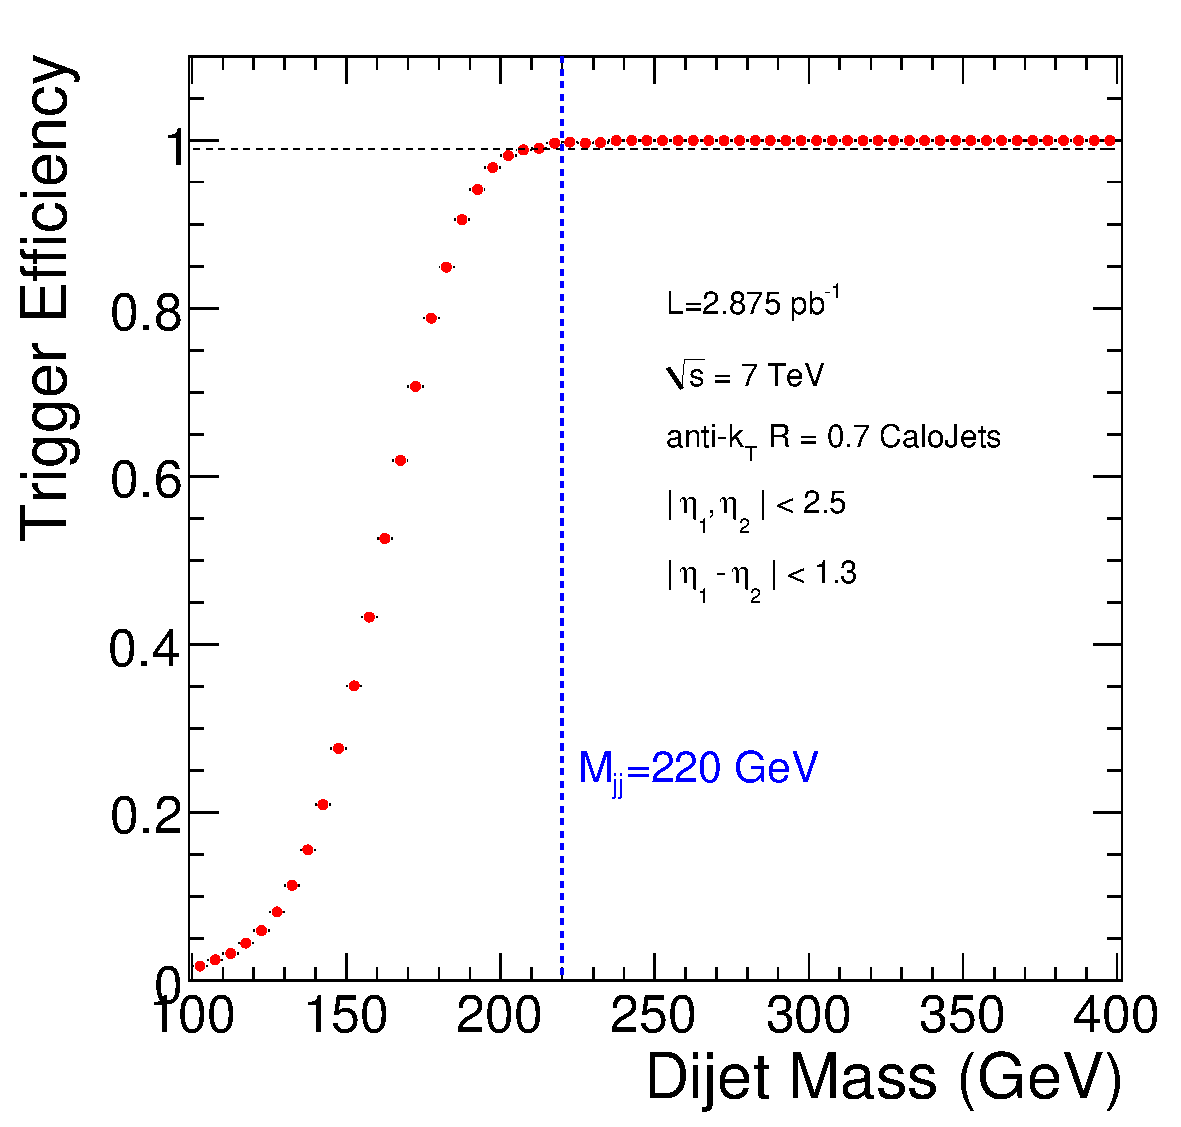
\includegraphics[width=0.6\textwidth]{Figures/HLT_Jet50U.pdf}
    \caption{ HLT\_Jet50U trigger efficiency as a function of dijet mass for 
    $|\eta|<1.3$ is measured from the data.}
    \label{Trigger}
  \end{center}
\end{figure}


The number of events vs. dijet mass are shown in figure~\ref{MassCut}.  The trigger turn over of the 
 HLT\_Jet50U trigger can be seen in the mass spectrum along with the 99\% efficiency ponit at 
 a mass of 210 GeV.  The processed dijet 
cut of 100 GeV has been relaxed to make this plot.

\begin{figure}[!ht]
  \begin{center}
    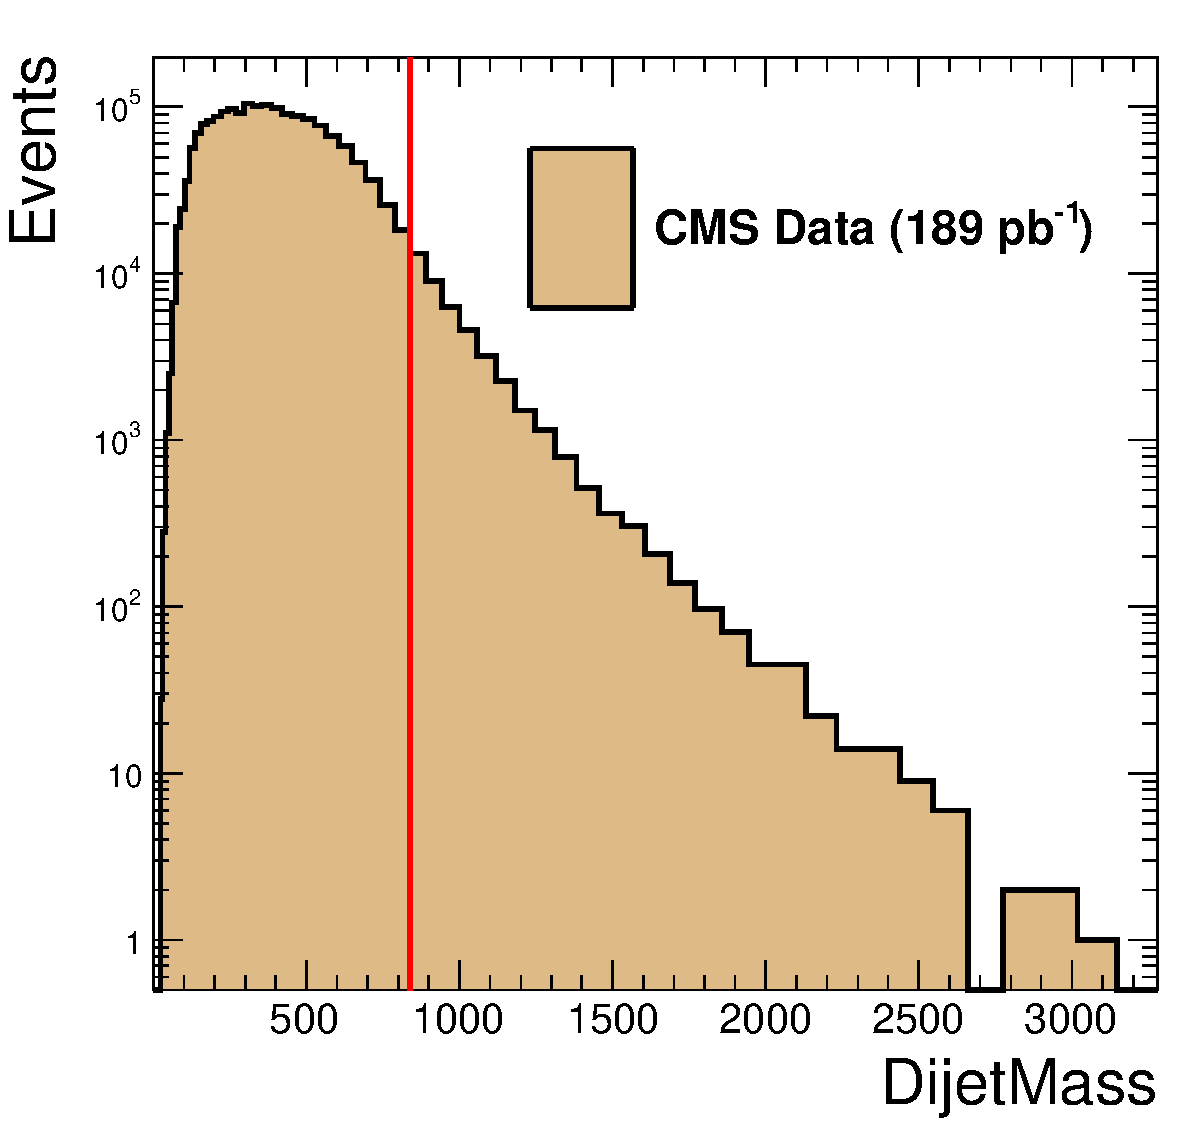
\includegraphics[width=0.6\textwidth]{Figures/c_DijetMass.pdf}
   \caption{ Number of events vs. dijet mass in GeV (histogram) requiring all cuts except the final dijet mass cut for trigger
   efficiency at $m=220$ GeV (vertical line)}
    \label{MassCut}
  \end{center}
\end{figure}
\clearpage
\subsubsection{Dijet Data Quality}

The number of events in the analysis after the basic cuts are shown for
each cut in table~\ref{table:cuts}
\begin{table}[th]
  \centering
  \normalsize
  \begin{tabular}{|l|r|}
    \hline
      Events after vertex cut                              &  6125930\\
      Events after dijet eta cuts: $|\Delta\eta|<1.3$ and $|\eta|<2.5$ & 2088922 \\
      Events after dijet mass cut: $m>200$ GeV & 414645 \\
      Events after jet id cut                              &   414131 \\
    \hline
  \end{tabular}
  \caption{Cuts and Events}
  \label{table:cuts}
\end{table}

The fraction of events rejected by Jet ID is very small, because the requirement that the
two leading jets have a dijet mass $m>220$ GeV, $|\eta|<2.5$ and $|\Delta\eta|<1.3$ enhances the jet purity.
514 events are rejected by jet ID. We have scanned all events rejected by Jet ID that have a dijet
mass of greater than 1.4 TeV, and they are all HPD noise that also has high $MET$, except for one 
event with a Sum $E_T$ of 400 TeV uniformly distributed across the HCAL.
%One event rejected by jet ID (run 139407 event 1102912914) has a jet with EMF of 0.009, but otherwise appears to be a good event with
%a dijet mass of $0.5$ TeV.
%One event rejected by Jet ID was in Event 156365648 in Run 135149, noise in a single RBX giving 
%two neighboring jets with EMF of 0 an event MET/$\Sigma E_T$=0.95. 
%A second event rejected by Jet ID was Event 217914565 in Run 135528, noise in  a single HPD,
%again giving two neighboring jets with EMF of 0 and fHPD of 1 and an event MET/$\Sigma E_T$=0.87.
%A third event rejected by Jet ID was Event 103871079 in Run 135175, in which the leading jet
%failed the EMF cut with $EMF=0.005$, but the event looks like it might be a real dijet event:
%jet 1 $p_T=74$ GeV, jet 2 $p_T=35$ GeV, $M_{JJ}=156.4$ GeV, tracks pointing at both jets, 
%$\Delta\phi=2.7$, and a marginal but passable MET/$\Sigma E_T$=0.24.  


After all cuts, we present some basic distributions indicating jet and event quality in 
Fig.~\ref{jet_id}, ~\ref{basic_event} and ~\ref{jet_kinematics}.


In Fig.~\ref{jet_id} we show the distributions of the variables of loose jet ID
after all cuts.  Jet EMF, the fraction 
of jet energy in the ECAL, does not have a peak near either zero or one which would indicate a 
problem from the
HCAL or ECAL. Loose jet ID requires jet EMF$ > 0.01$ and we find
that the cut rejects no real jets in dijet events as discussed above. Jet fHPD, the fraction of jet energy in 
the hottest HCAL HPD, does not have a peak near one which would indicate a problem from 
HPD noise.  Loose jet ID requires
jet fHPD$ < 0.98$.  Jet n90hits, the number of energy ordered HCAL and ECAL RecHits 
containing 90\% of the jet energy, does not have a peak near one which would indicate 
hot cells in the calorimeter for example from Ecal spikes.
Loose jet ID requires jet n90hits $> 0$.  Data and MC have
similar shapes and show smoothly 
varying distributions for jet EMF, fHPD, and n90hits 
characteristic of real jets.  These jet ID variables give us confidence 
that the jets in this analysis do not originate from backgrounds in the calorimeter.

In Fig.~\ref{track_multiplicity} we show the number of good tracks 
associated with either of the two leading jets.  Our leading jets generally have many 
associated tracks.  Very few of the leading jets, in both MC and data, have no 
associated tracks at the calo face, and there are virtually no leading jets without associated
tracks at the vertex. The track multiplicity distributions do not have a peak at zero tracks,
which would indicate calorimeter backgrounds.  The track multiplicity distribution gives 
us additional confidence that the calorimeter jets in this analysis come from pp collisions.

In Fig.~\ref{basic_event} we show some event balance distributions.  
The dijet events have low MET/$\Sigma E_T$,
the ratio of the magnitude of the vector and scalar sums of the CaloTowers,
indicating that the event energy is well balanced in the transverse plane. 
Large background from calorimeter noise, beam halo, or cosmic rays will typically
produced large values of MET/$\Sigma E_T$, which we do not observe in this data.
The handful of events with MET/$\Sigma E_T>0.5$ have been scanned, and they all look like good 
monojet events at dijet mass around $0.2-0.3$ TeV, most likely from 
$W(\mu \nu)$ + jet or $Z(\mu\mu, \nu\nu)$ + jet processes.
The two leading jets are predominantly back-to-back in $\phi$ as expected for 
dijets, with a tail to small values of $\Delta\phi$ produced by radiation 
and multi-jet events. 
Data and MC have similar shapes and show 
smoothly varying distributions for  MET/$\Sigma E_T$ and $\Delta\phi$ 
characteristic of dijet events. Thes distributions give us confidence
that we are observing events with a dijet topology, not unphysical backgrounds.


In Fig.~\ref{jet_kinematics} we show some distributions of basic jet
kinematic variables.  The $p_T$ distribution falls steeply with increasing
$p_T$, and turns over at low $p_T$ due to the dijet mass cut $m>354$ GeV.
The jet $p_T$ distributions for data and MC are in good agreement considering
uncertainties in the jet energy scale, discussed in section~\ref{JESerror}, 
and the modelling of the $p_T$ distribution
in PYTHIA.
The $\eta$ distribution of the two leading jets is in reasonable agreement with 
the shape predicted by the MC, and there are no regions with significant
rate deviations that could arise due to significant mis-understanding of jet response
after all corrections. The $\Delta\eta$ distribution demonstrates the 
characteristic forward peaks from Rutherford-like QCD scattering at 
fixed invariant mass, and the very slight deviations in shape between
data and MC are expected from NLO effects on the angular distribution.
The $\phi$ distribution of the two leading jets is flat, with an RMS of
only 2.2\%, which corresonds to a CaloJet response which is flat as a function of phi 
to within about 0.4\%, which is reasonable given expected calorimeter response uniformity in $\phi$. 
The $\eta$ - $\phi$ distribution of two leading jets is reasonably uniform and 
does not show any indication of hot or dead regions of the calorimeter. 
These distributions show that the jets in this data sample 
have the kinematics expected for dijets from QCD.

\begin{figure}[!ht]
  \begin{center}
    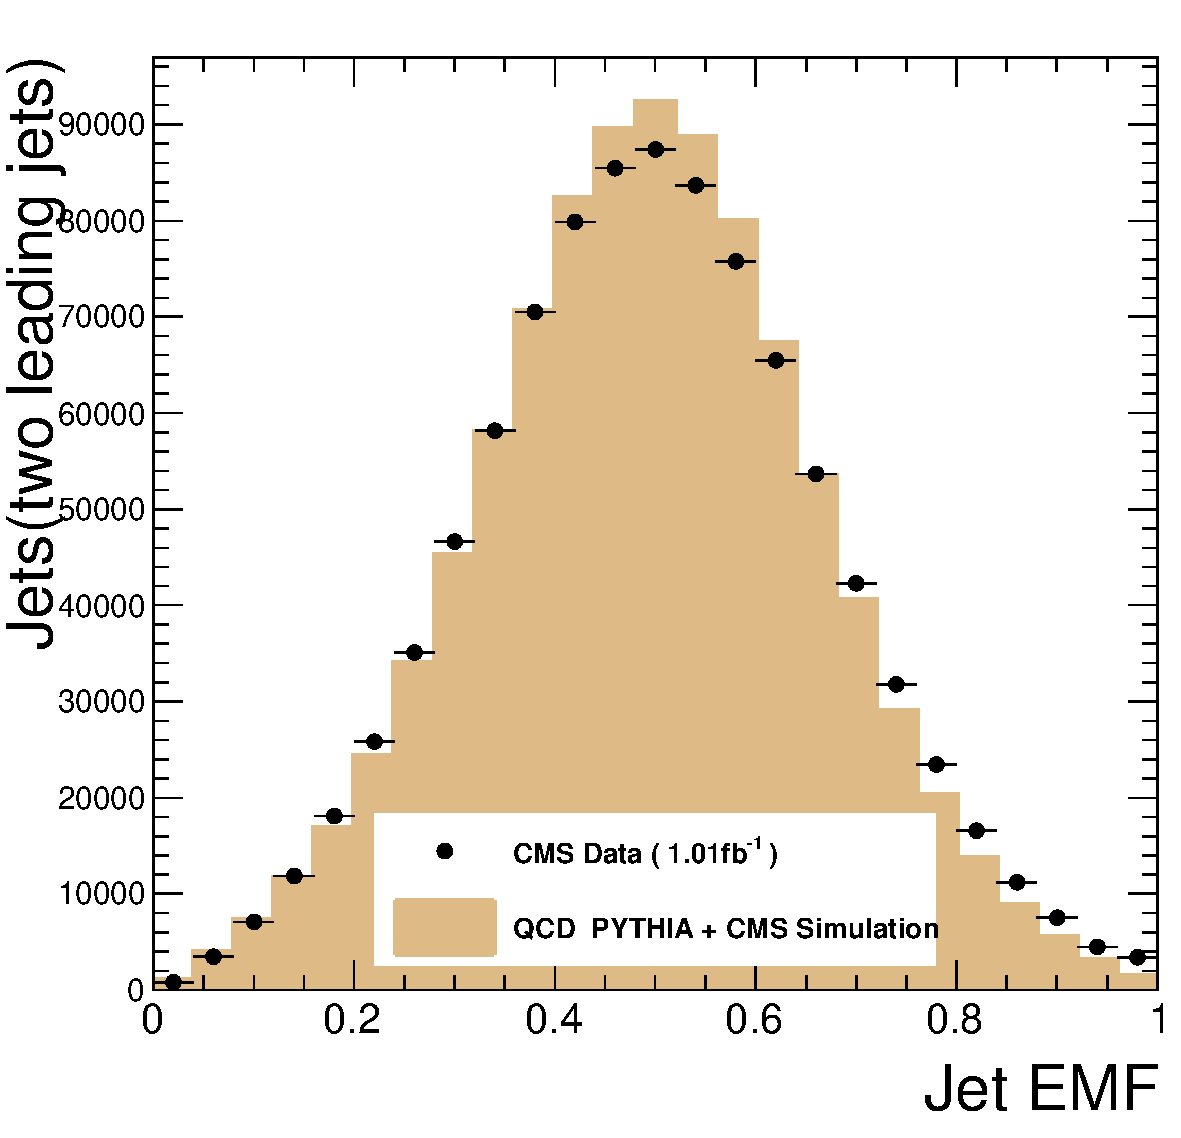
\includegraphics[width=0.45\textwidth]{Figures/c_EMF.pdf}
    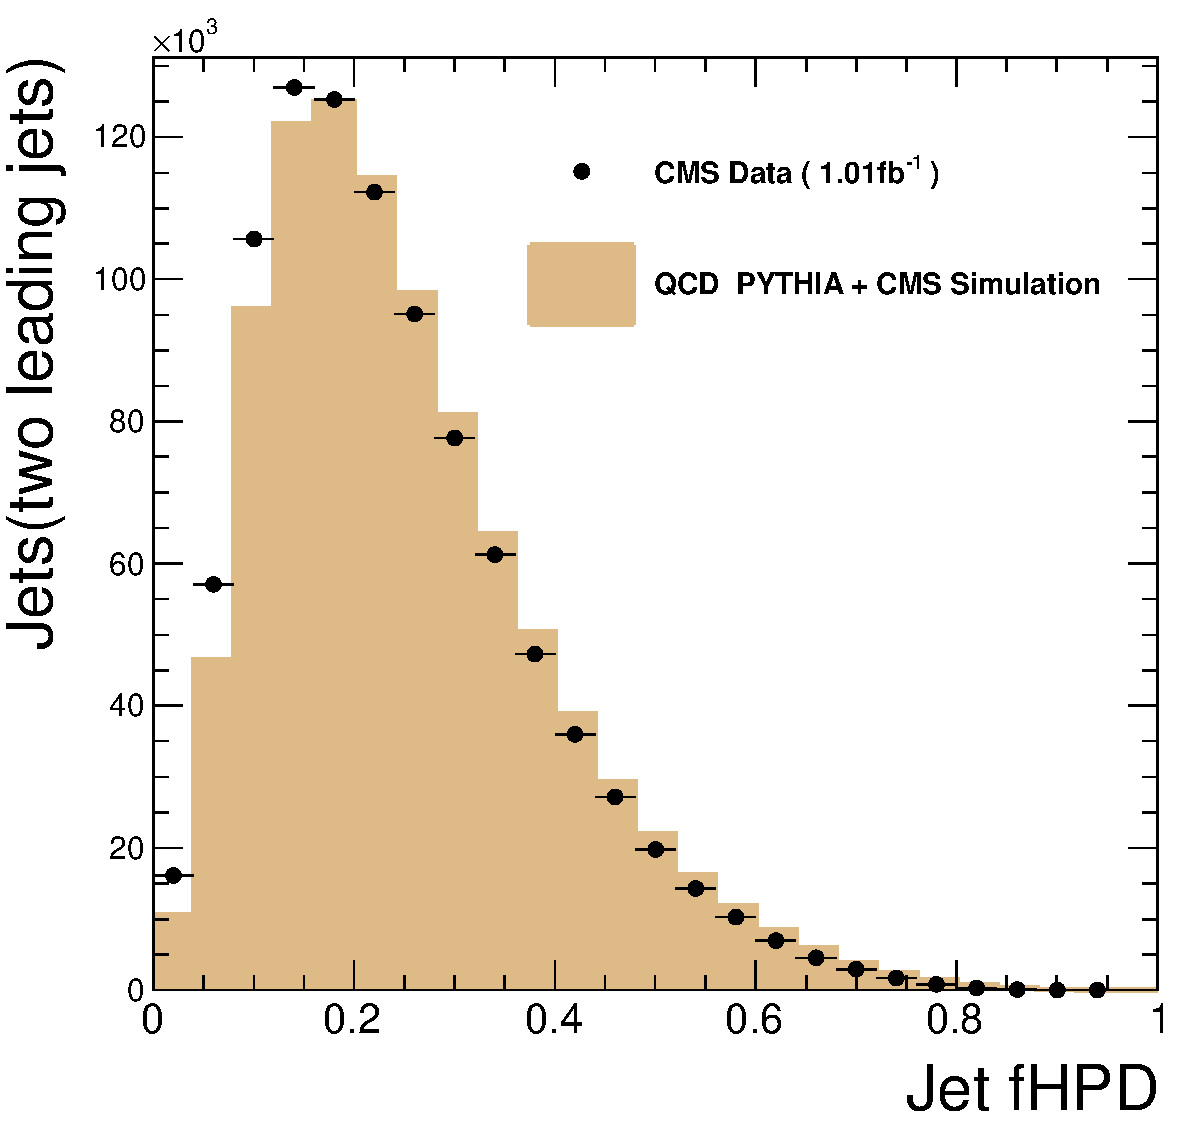
\includegraphics[width=0.45\textwidth]{Figures/c_fHPD.pdf}
    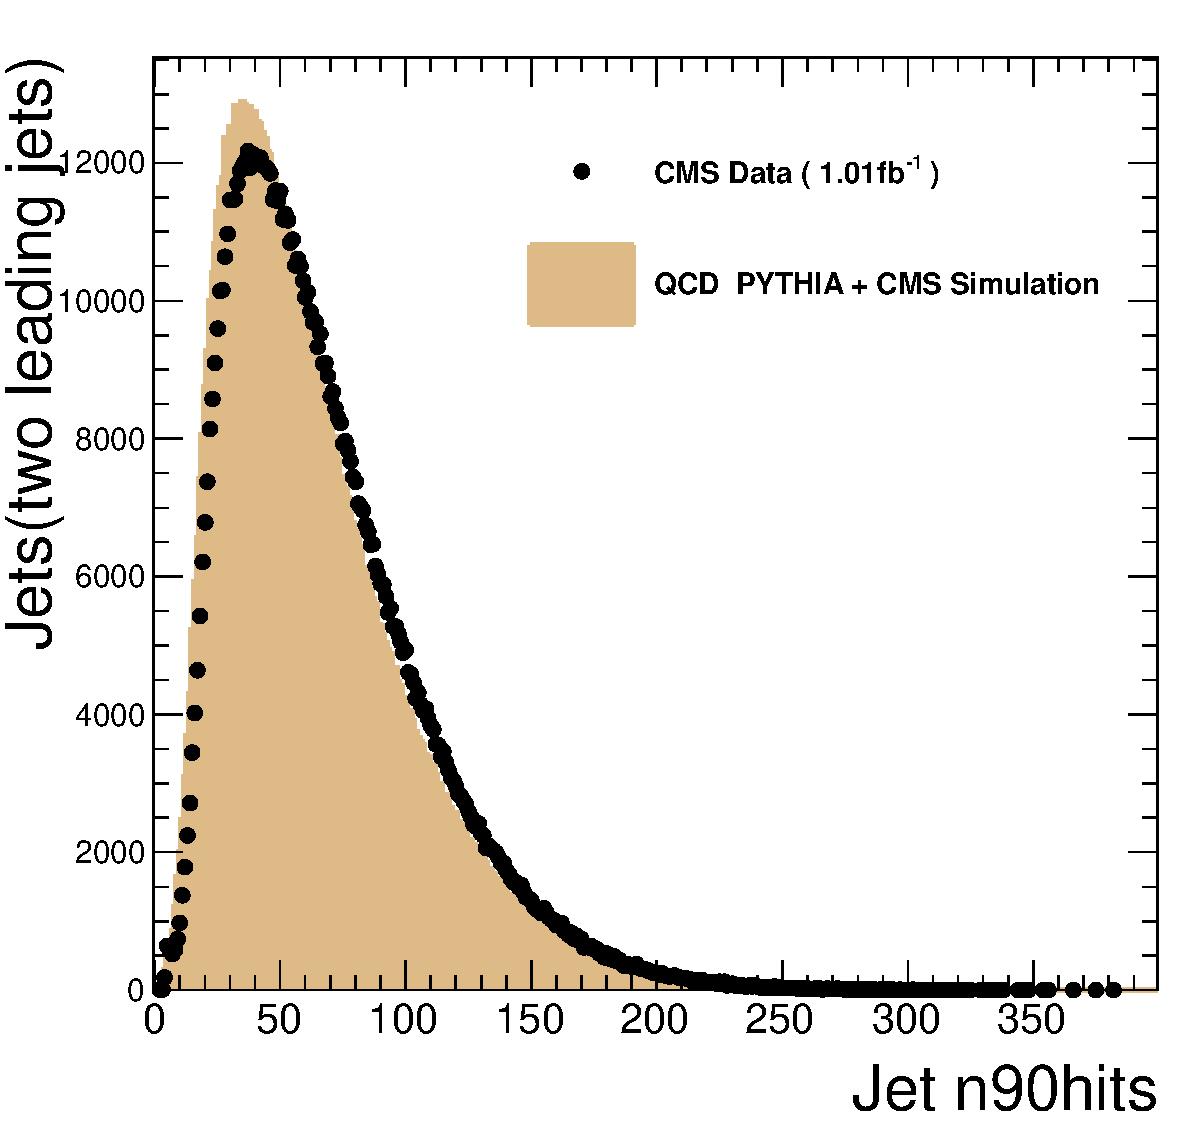
\includegraphics[width=0.45\textwidth]{Figures/c_n90hits.pdf}
    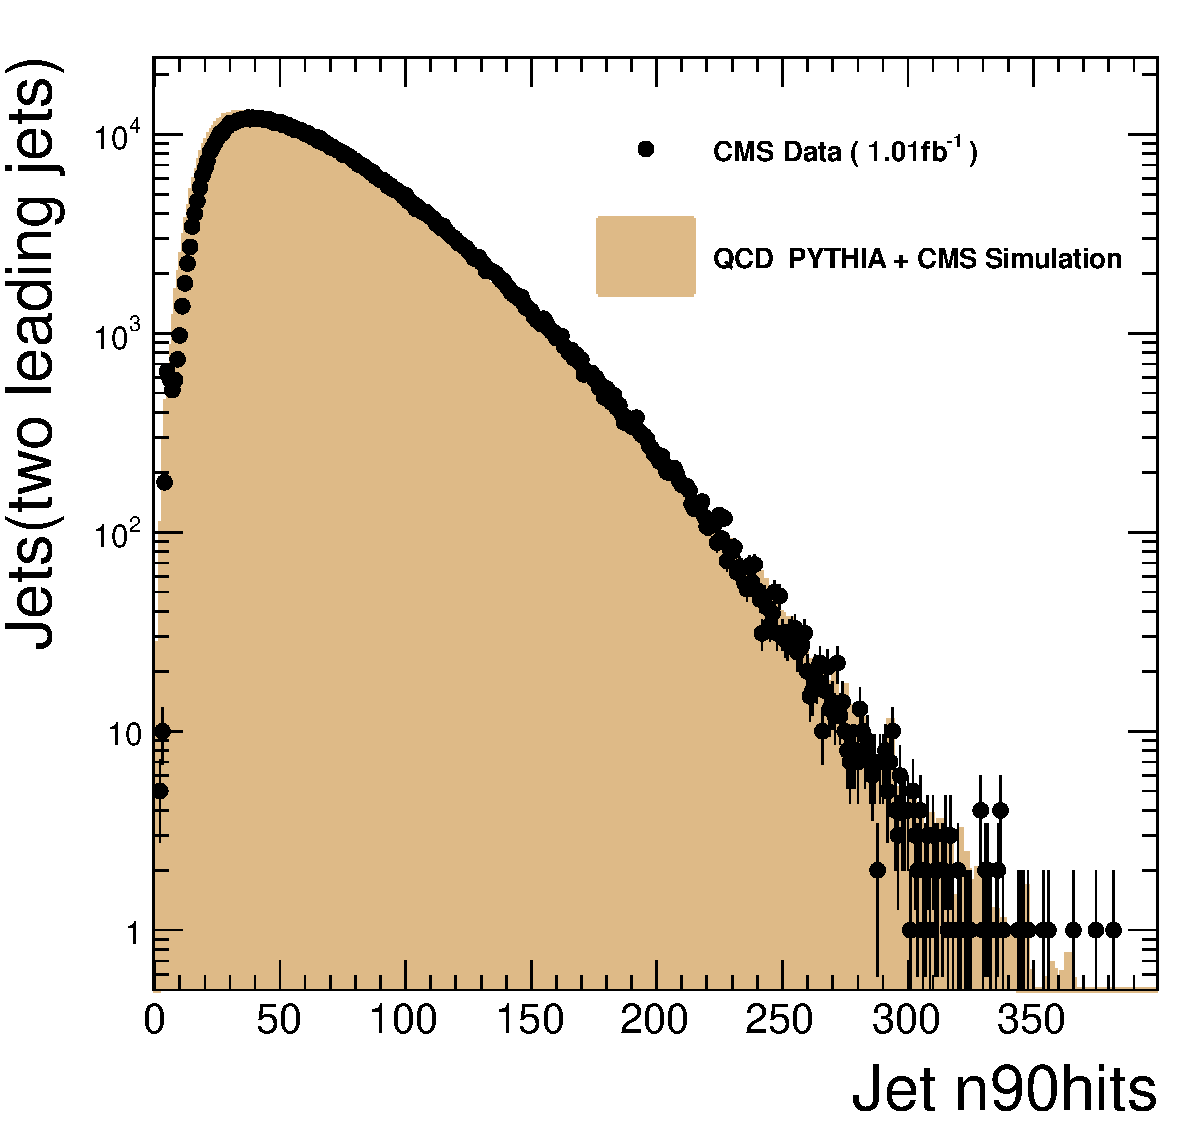
\includegraphics[width=0.45\textwidth]{Figures/c_n90hits_log.pdf}

    \caption{Jet ID Distributions.  The EM
      energy fraction of the two leading jets (upper left), the fHPD for the two
      leading jets (upper right), the n90hits for the two leading jets
      (lower left) and the same in log scale
      (lower right). }
    \label{jet_id}
  \end{center}
\end{figure}

\begin{figure}[!ht]
  \begin{center}
    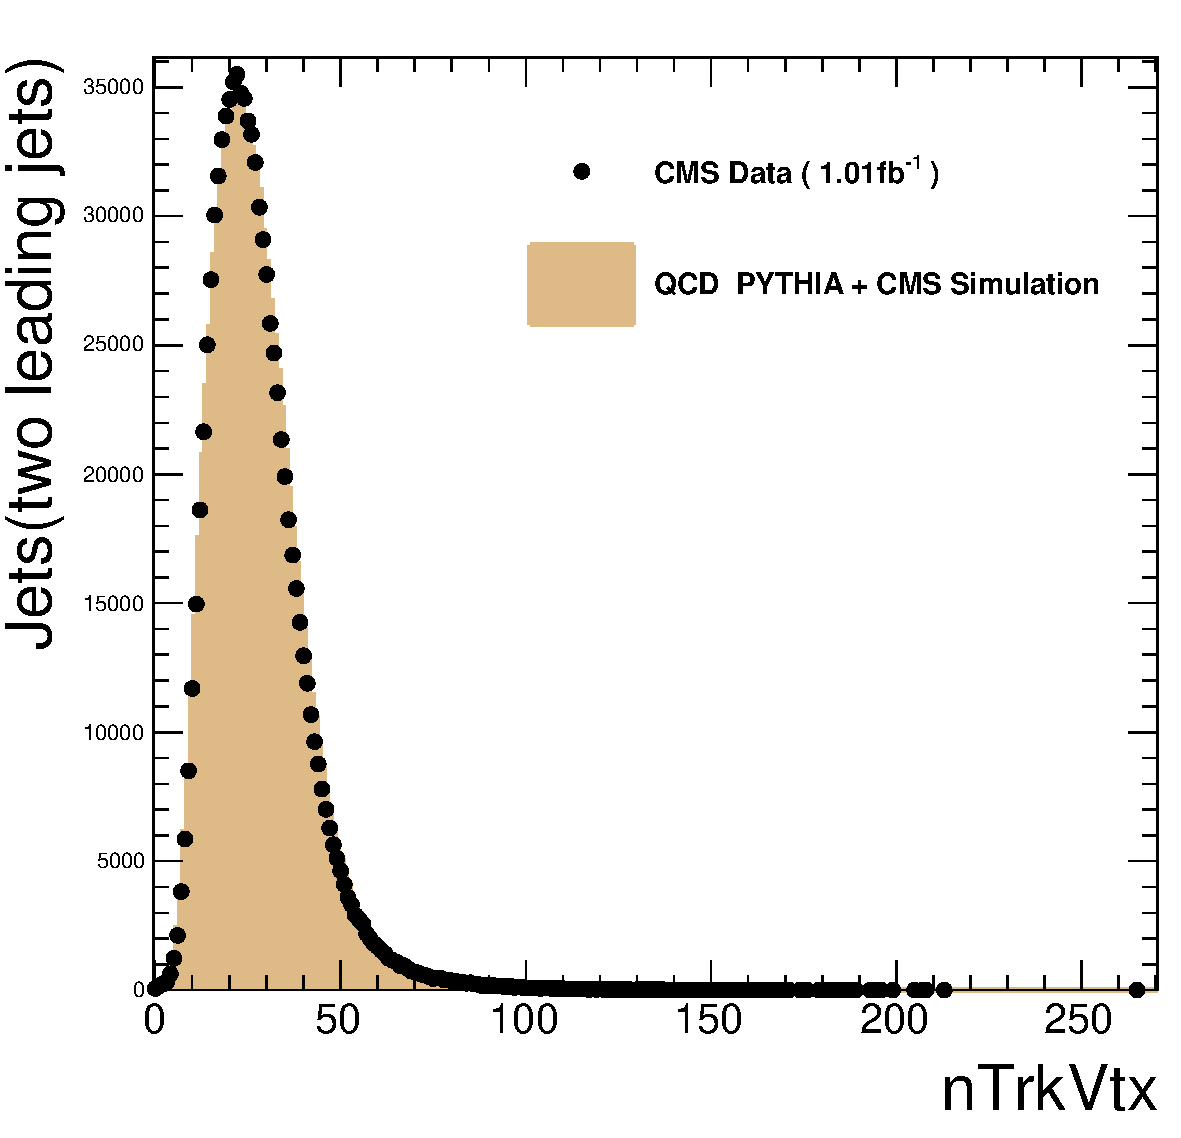
\includegraphics[width=0.45\textwidth]{Figures/c_nTrkVtx.pdf}
    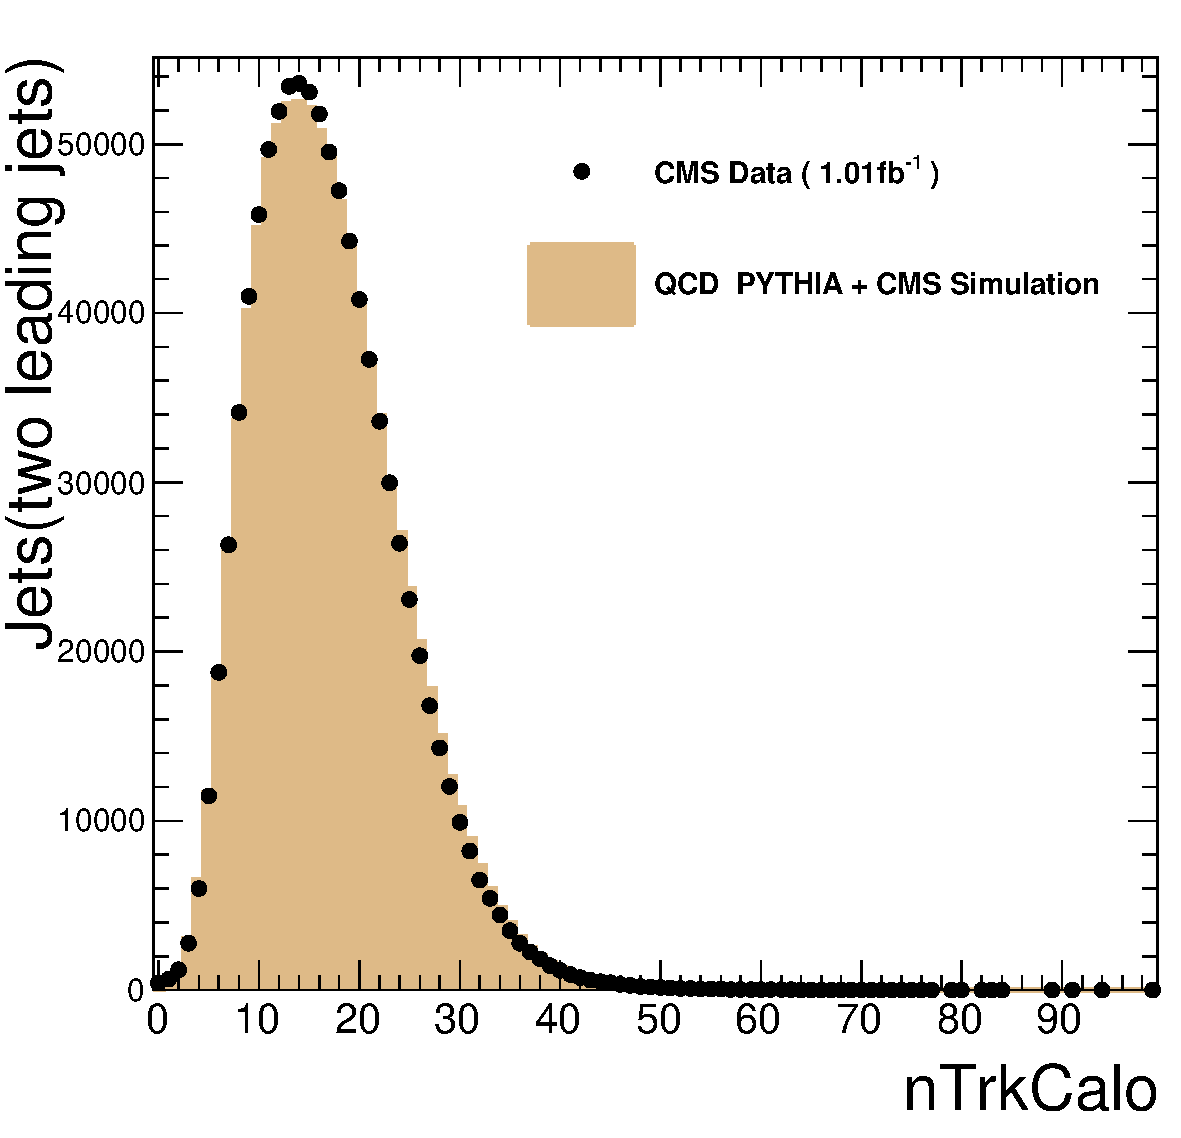
\includegraphics[width=0.45\textwidth]{Figures/c_nTrkCalo.pdf}
    \caption{ left) The multiplicity of tracks associated to two leading jets at the vertex right) The multiplicity of tracks associated to two leading jets at the calo face}
    \label{track_multiplicity}
  \end{center}
\end{figure}

\begin{figure}[!ht]
  \begin{center}
   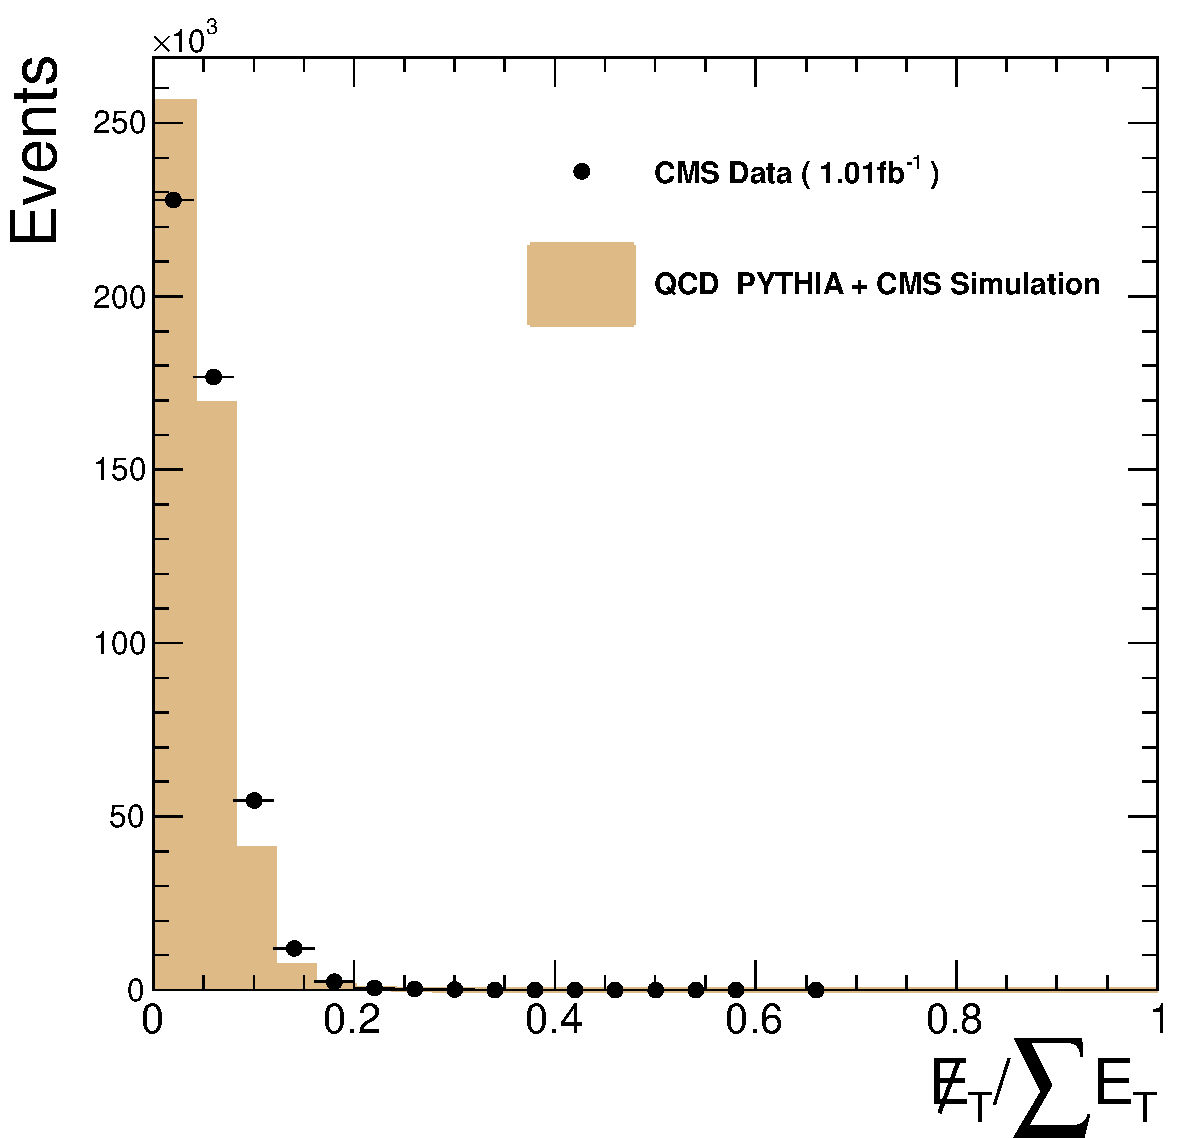
\includegraphics[width=0.45\textwidth]{Figures/c_MET_over_sumEt.pdf}
   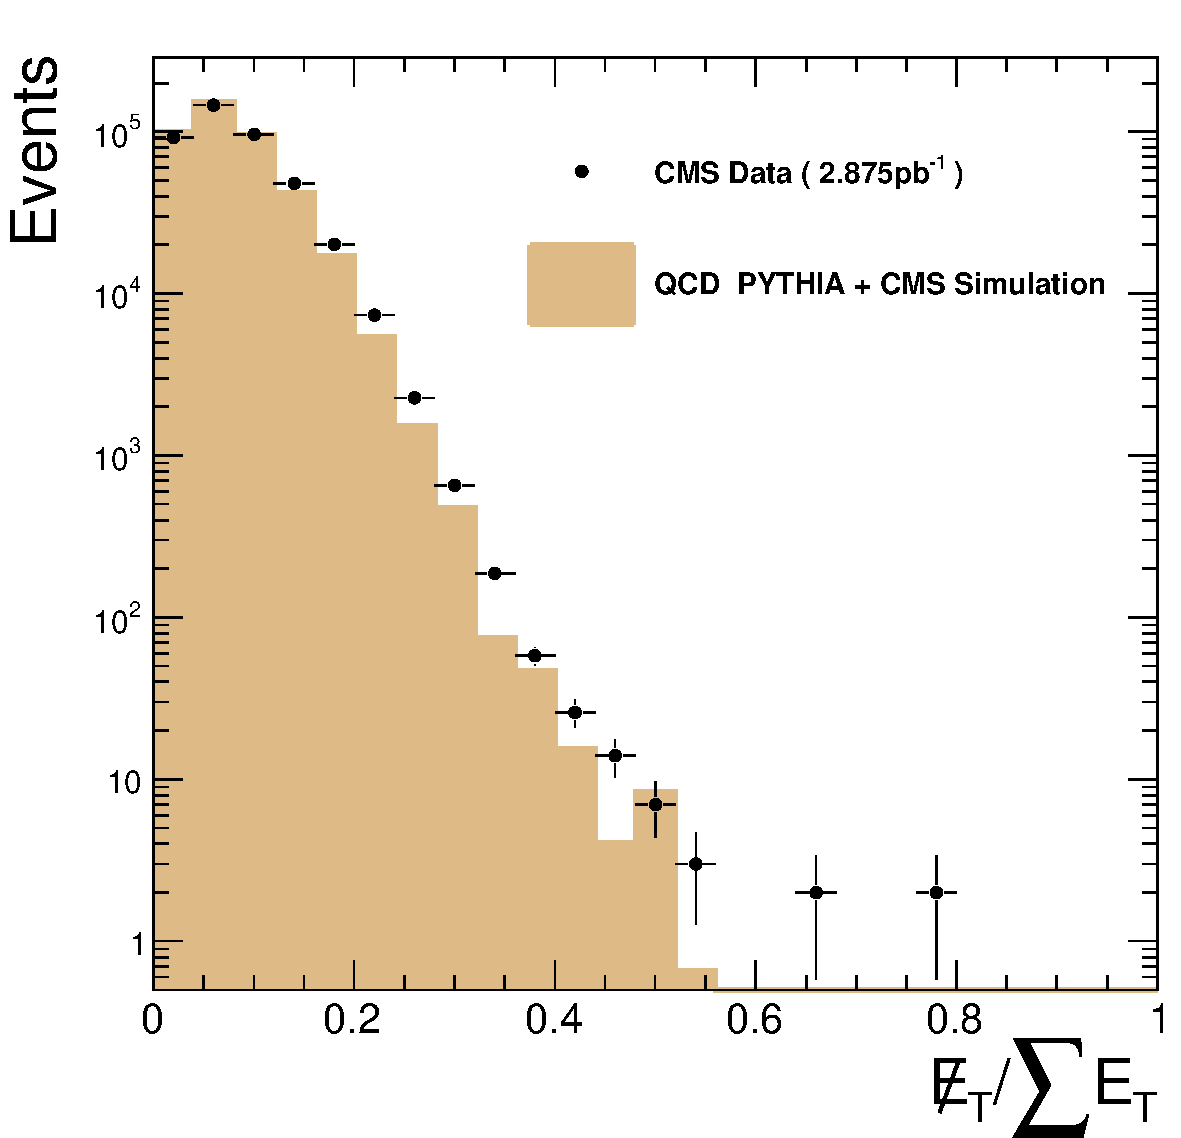
\includegraphics[width=0.45\textwidth]{Figures/c_MET_over_sumEt_log.pdf}
   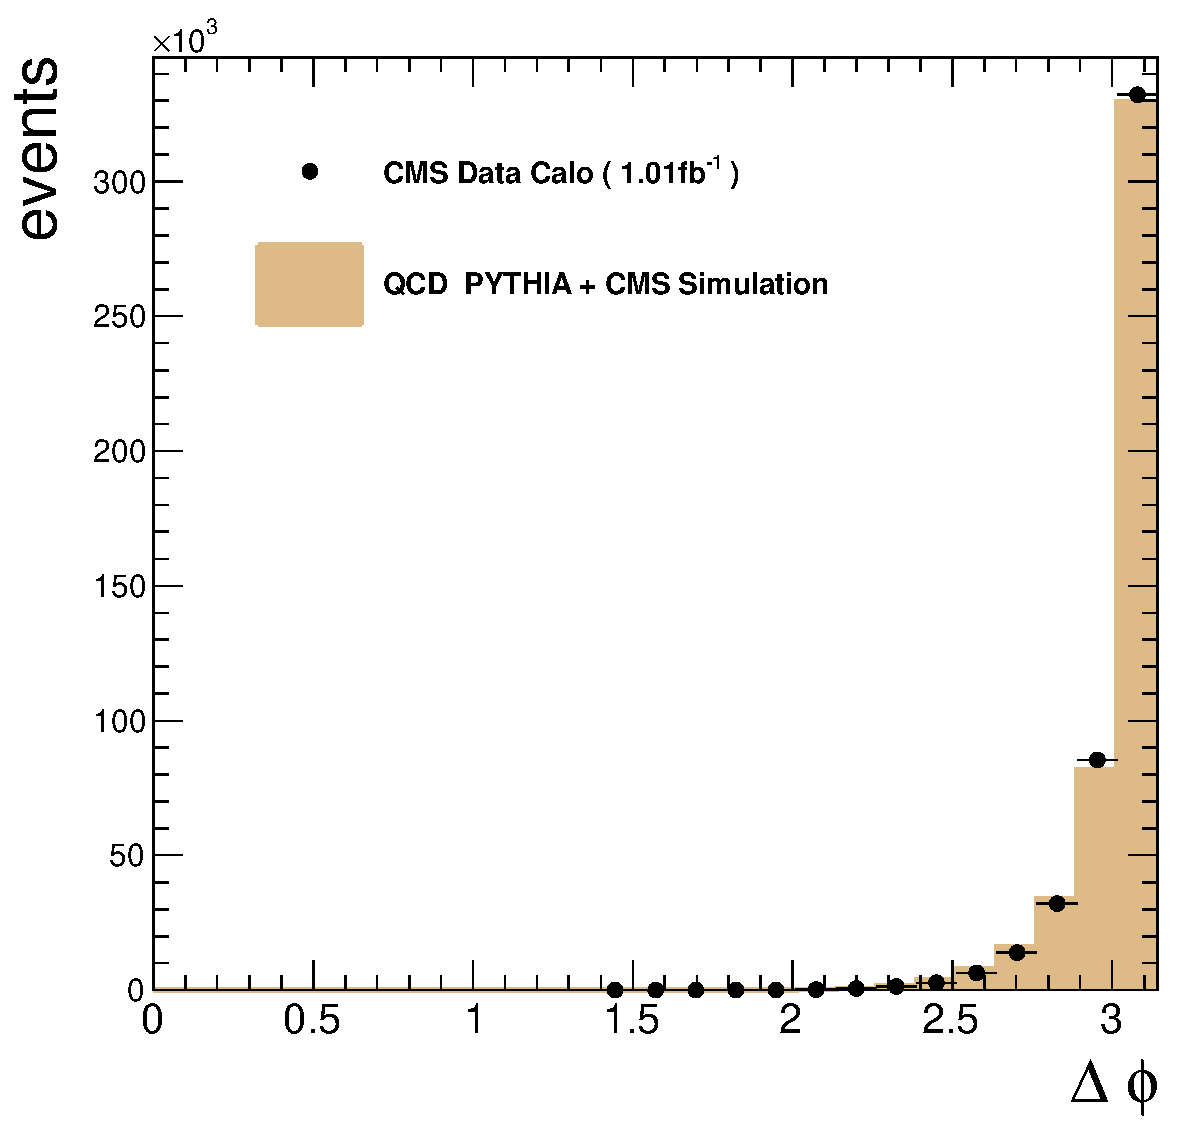
\includegraphics[width=0.45\textwidth]{Figures/c_DPhi.pdf}
   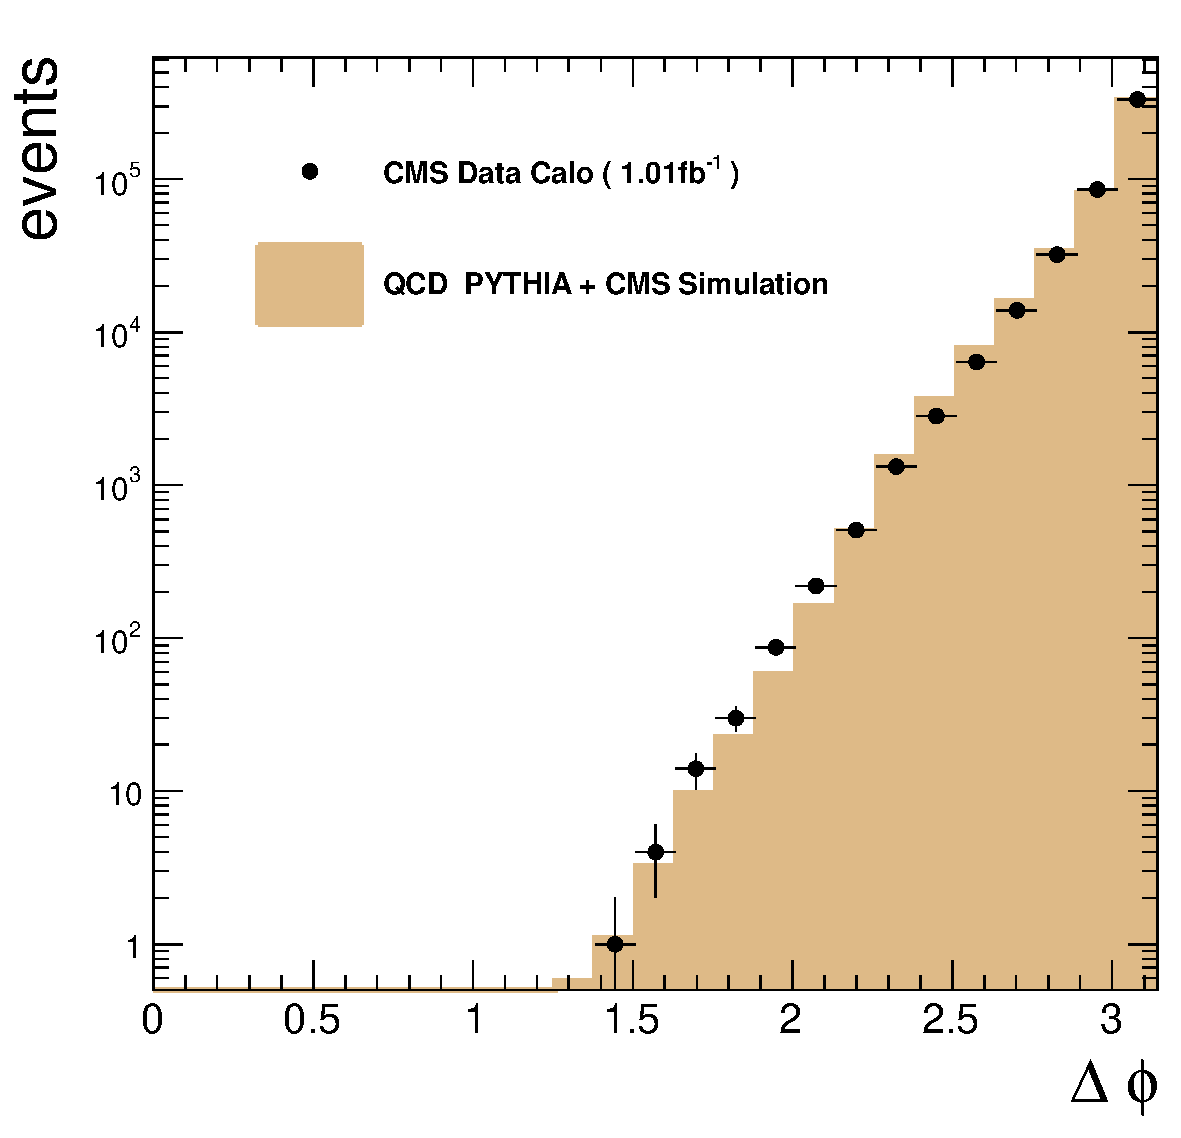
\includegraphics[width=0.45\textwidth]{Figures/c_DPhi_log.pdf}

   \caption{ Event balance distributions.  Missing
    calorimeter $E_T$ divided by total calorimeter $E_T$ 
    (upper left) and the same in log scale (upper right).
    The $\phi$ difference of the two leading jets (lower left) 
    and the same in log scale (lower right).}
    \label{basic_event}
  \end{center}
\end{figure}


\begin{figure}[!ht]
  \begin{center}
    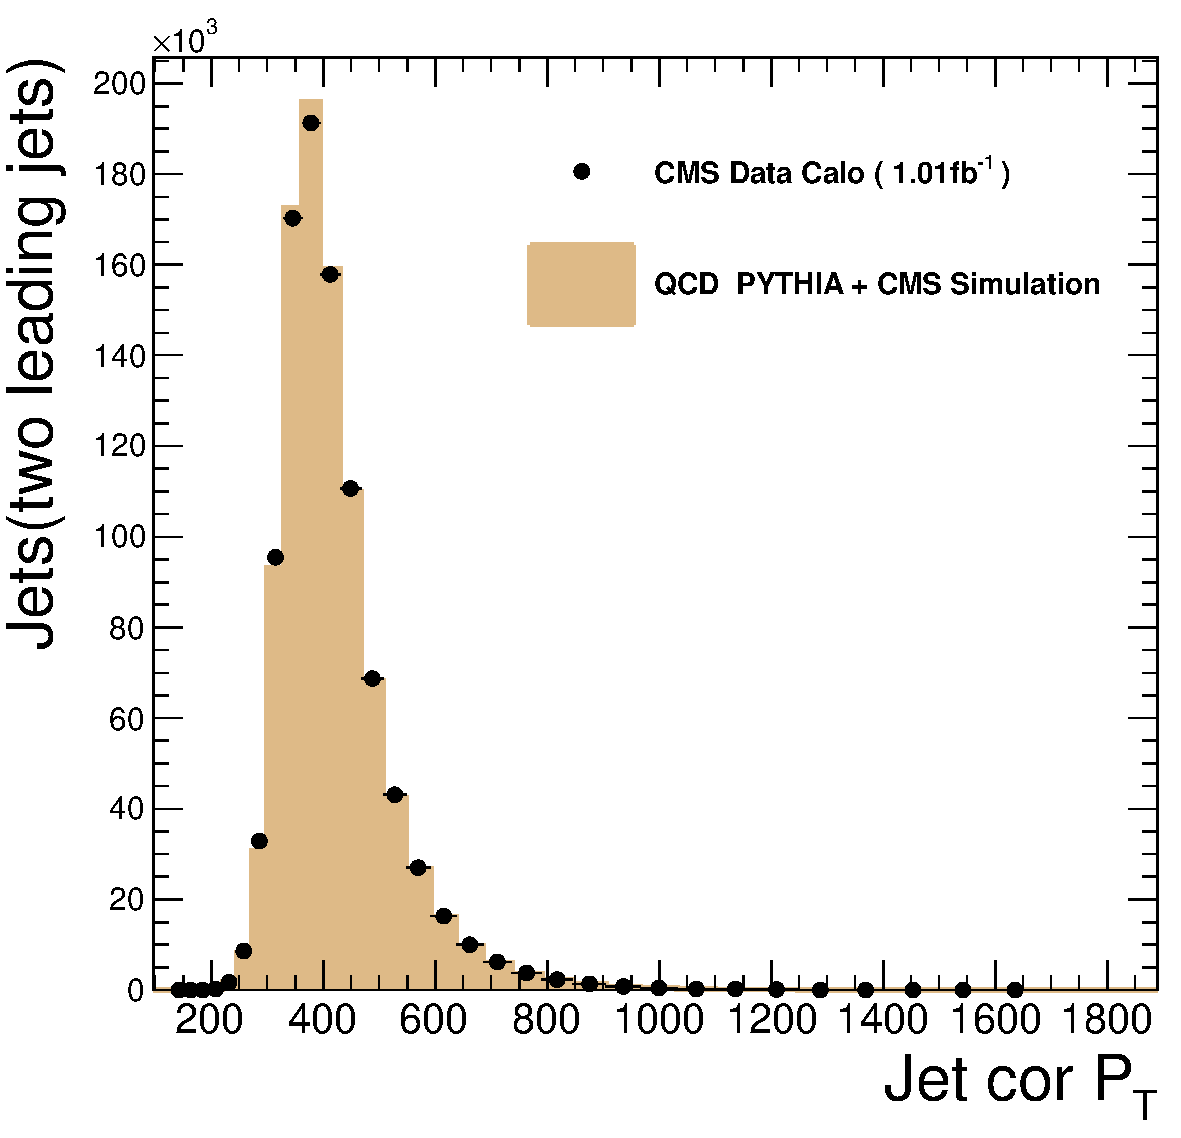
\includegraphics[width=0.45\textwidth]{Figures/c_corPt.pdf}
    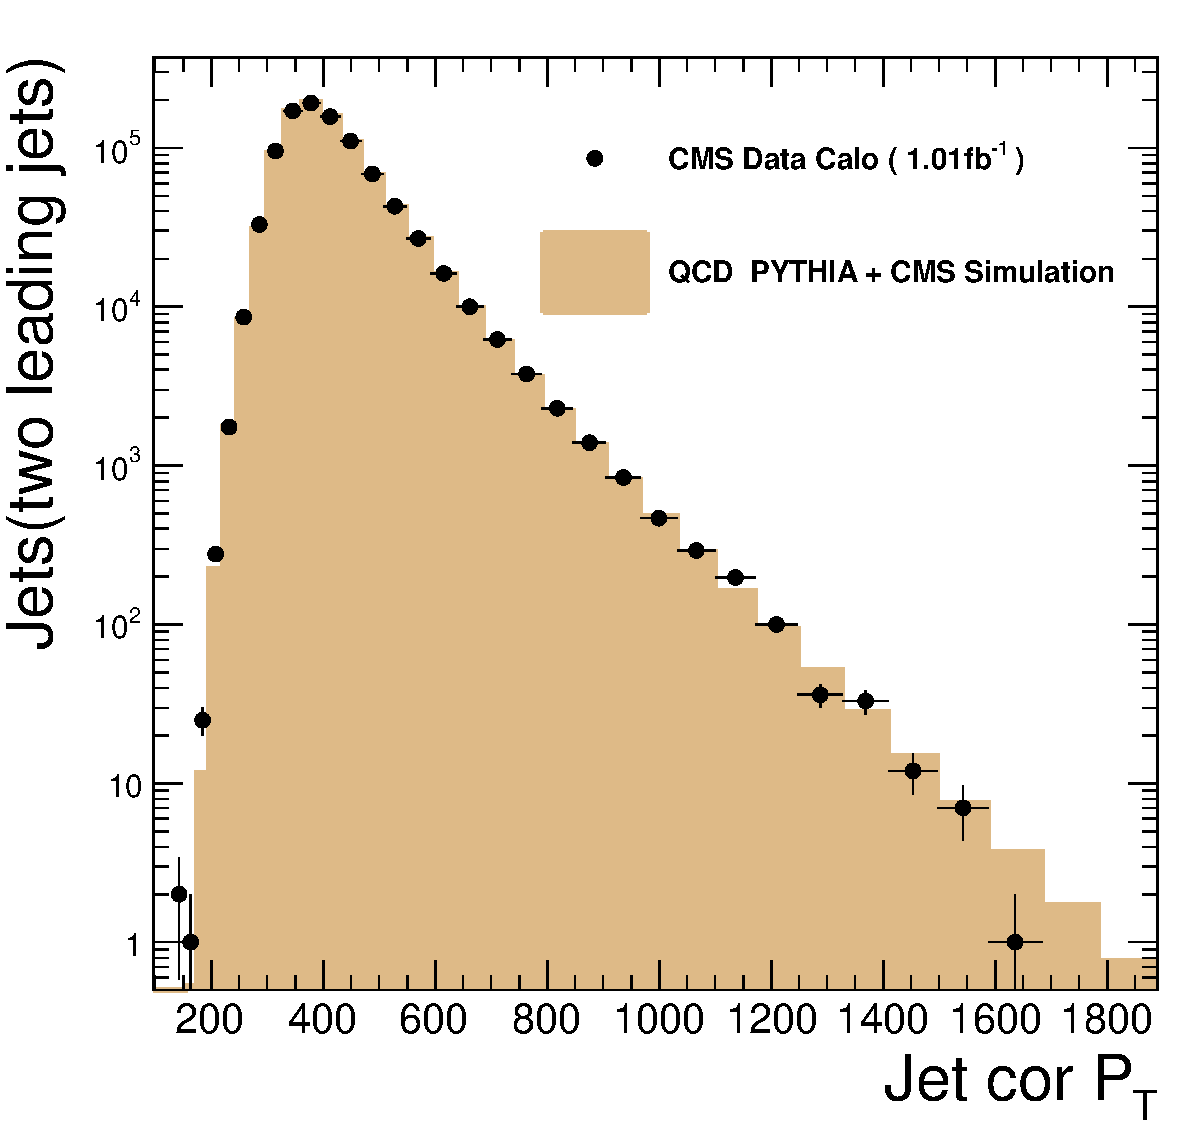
\includegraphics[width=0.45\textwidth]{Figures/c_corPt_log.pdf}
    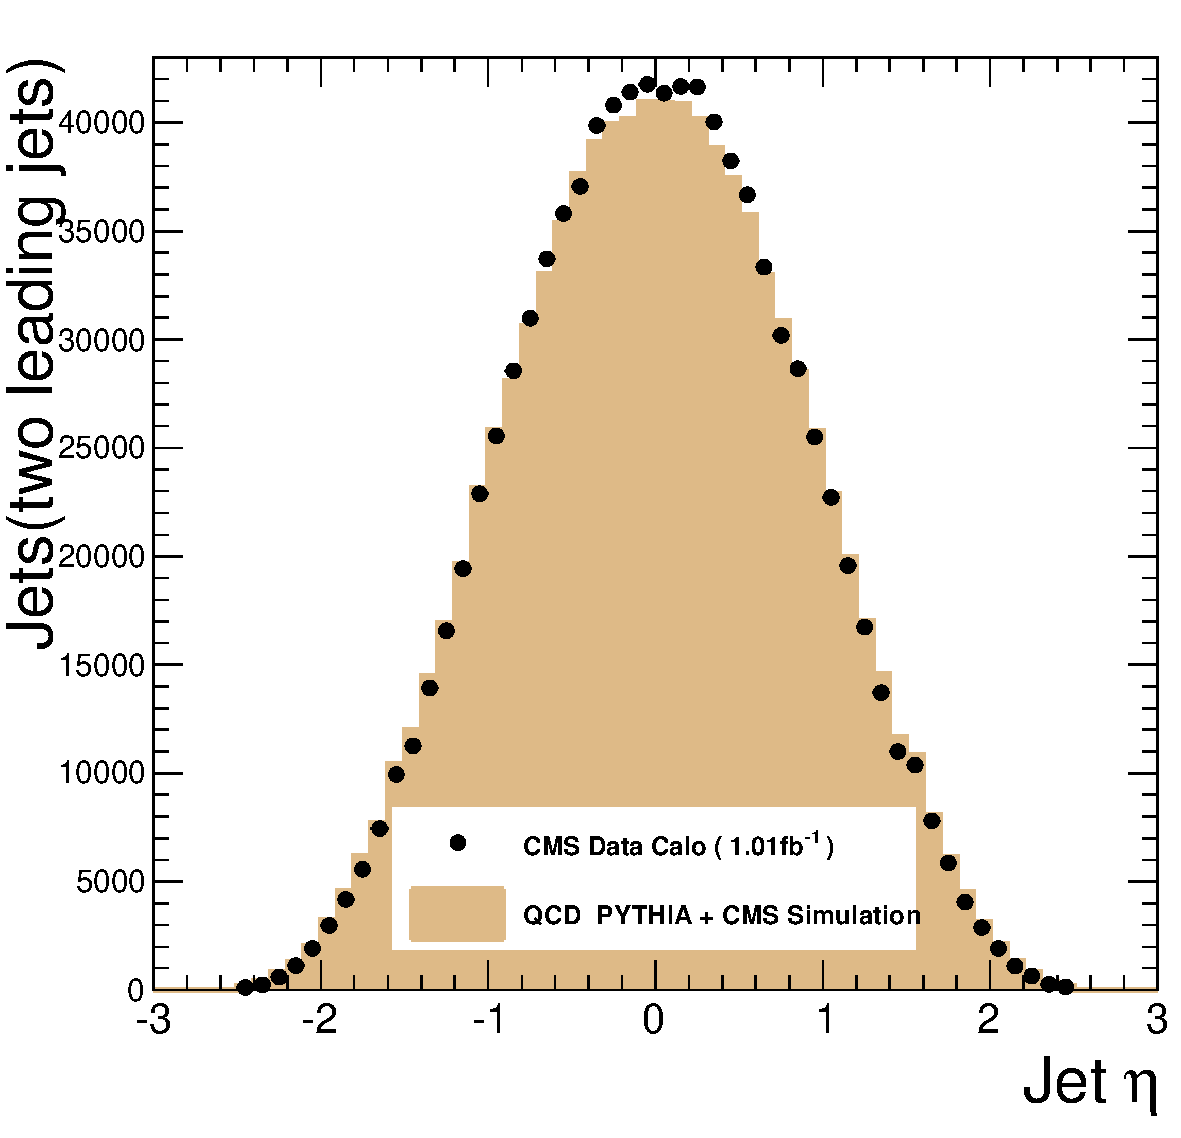
\includegraphics[width=0.45\textwidth]{Figures/c_Eta.pdf}
    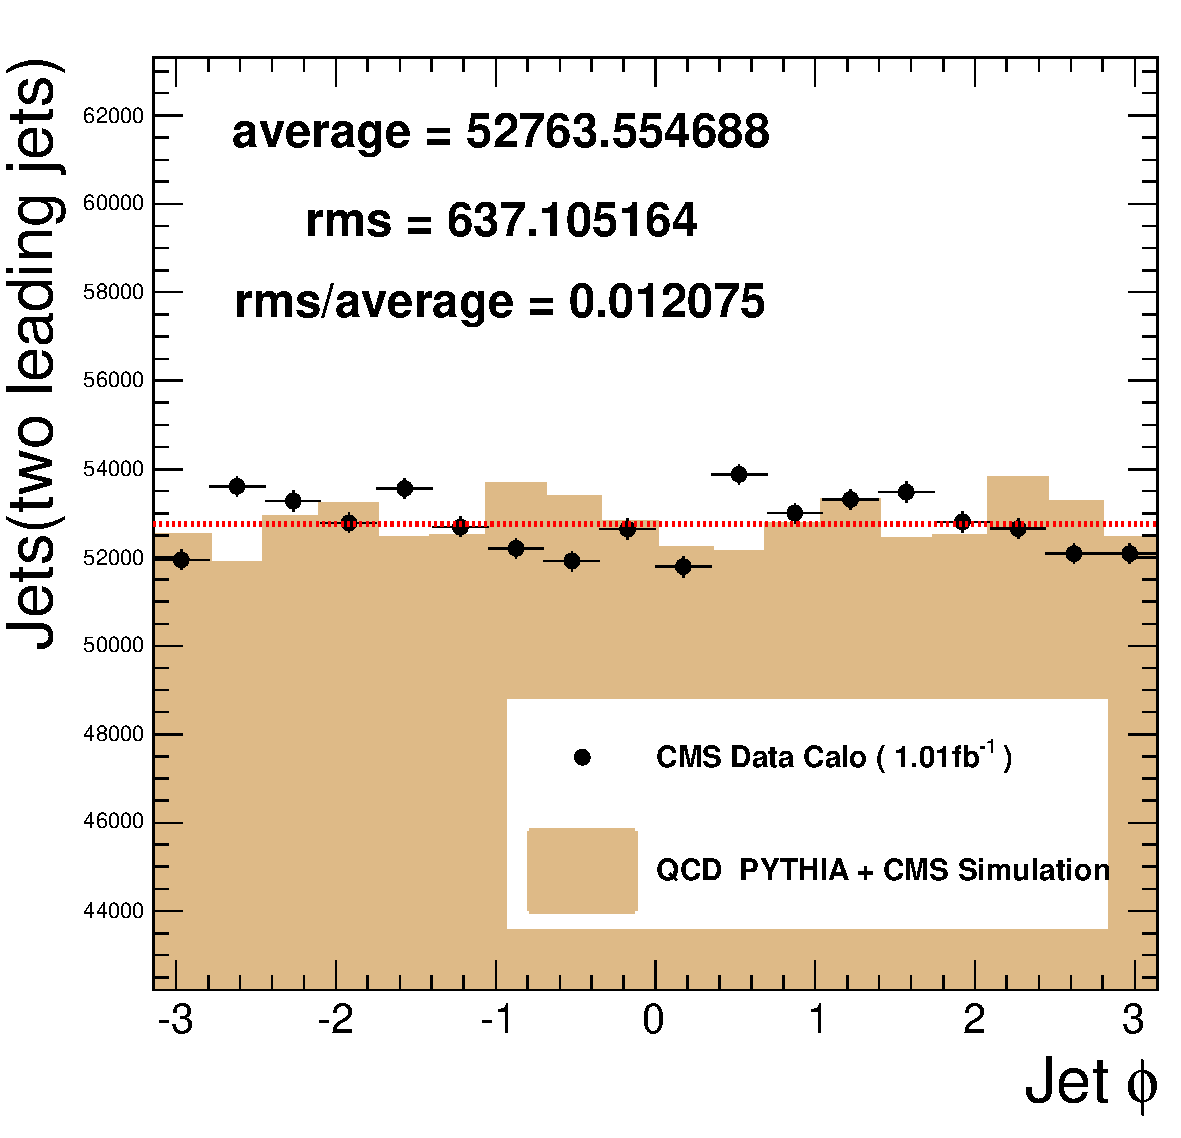
\includegraphics[width=0.45\textwidth]{Figures/c_Phi.pdf}
    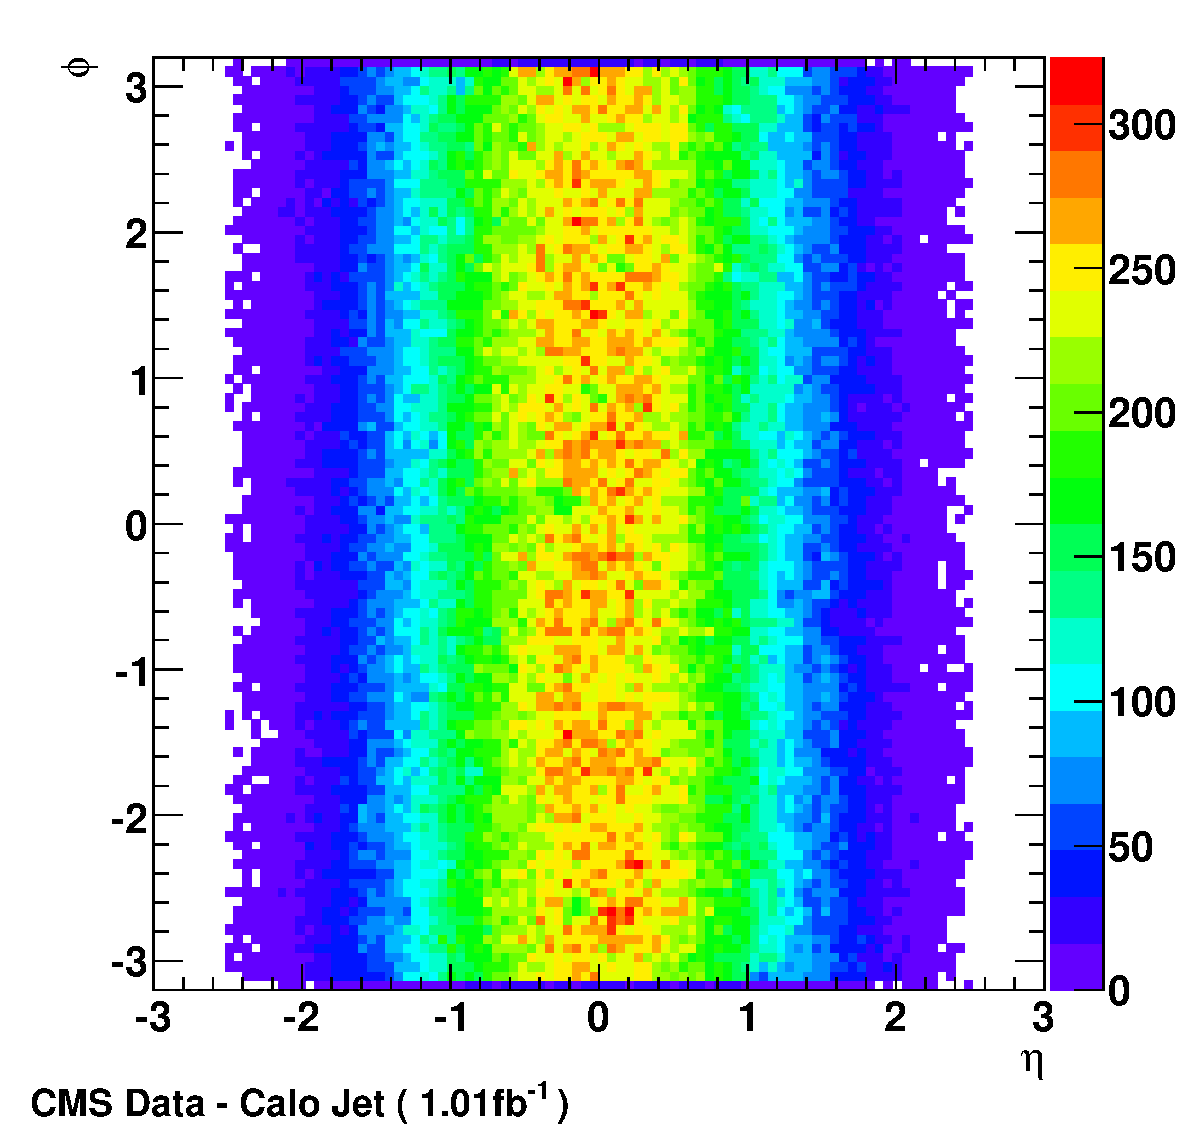
\includegraphics[width=0.45\textwidth]{Figures/c_Eta_Phi_Scatter.pdf}
    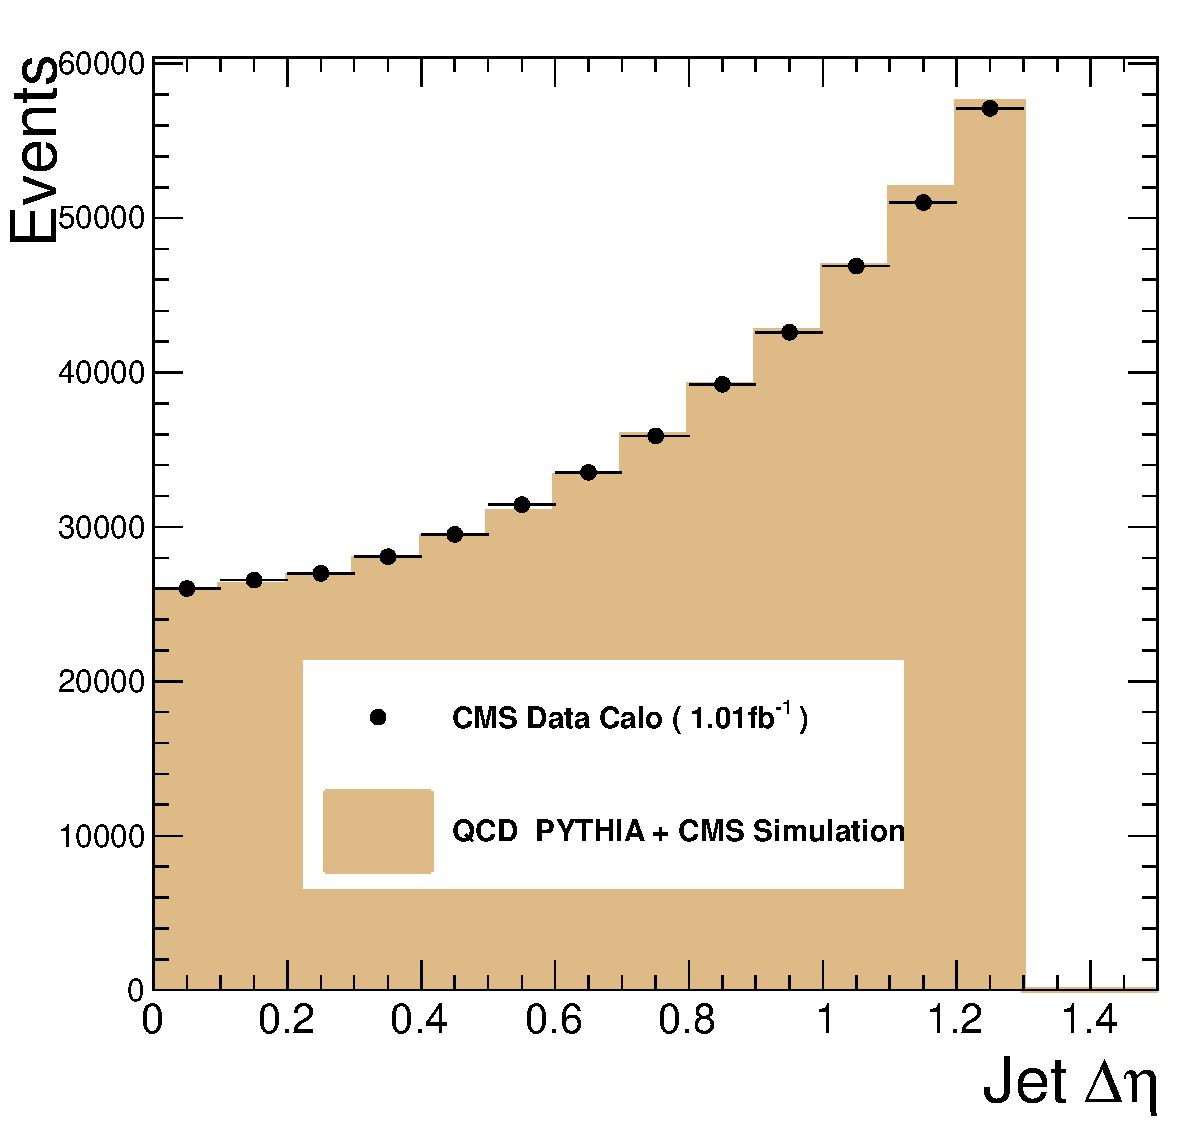
\includegraphics[width=0.45\textwidth]{Figures/c_DEta.pdf}

    \caption{ Jet kinematics distributions.  The corrected 
      $P_T$ of the two leading jets (upper left) and the same in log scale
      (upper right). The $\eta$ distribution for the
      two leading jets (middle left). The $\phi$ distribution for the two leading jets. (middle right)
      $\phi$ vs. $\eta$ (lower left) for the two leading jets. The $\Delta\eta$ distribution (lower right) }
    \label{jet_kinematics}
  \end{center}
\end{figure}


\subsubsection{Dijet Data Stability}

In order to demonstrate the stability of our data as a function of run, we show various event
and jet related quantities. In Fig.~\ref{MassVsRun} we show the number of dijet events surviving 
the full selection, for each run used in the analysis. We also show the mean dijet mass vs. run. 
In Fig.~\ref{XsecVsRun}, we show the number of dijet events divided by the integrated luminosity
of each run, vs. run. The observed cross-section is well behaved and very stable with an RMS of 
only 2\%.
%, with $\sim 20\%$ fluctuation around
%the weighted average primarily due to low number of events per run; 
A minimum
luminosity of 1 nb$^{-1}$ in each 
run is required for the plot. The cross-section as a function of run is  very 
sensitive to the jet energy scale stability which in turn is sensitive to the 
the calibration of the calorimeter. A change of just 0.4\% in the jet energy scale between
one run and the next would produce a change of around 2\% in the observed cross
section.  In addition, the cross-section is sensitive to the luminosity 
evaluation.  The observed stability of the cross section is an indication of a stable calorimeter energy 
scale and luminosity evaluation.

In Fig.~\ref{JetPropertiesVsRun} we show the mean value of the basic jet properties (\pt, EMF, number of
associated tracks), separately for the two leading jets, vs. run. Good stability is observed for all observables.

\begin{figure}[!ht]
  \begin{center}
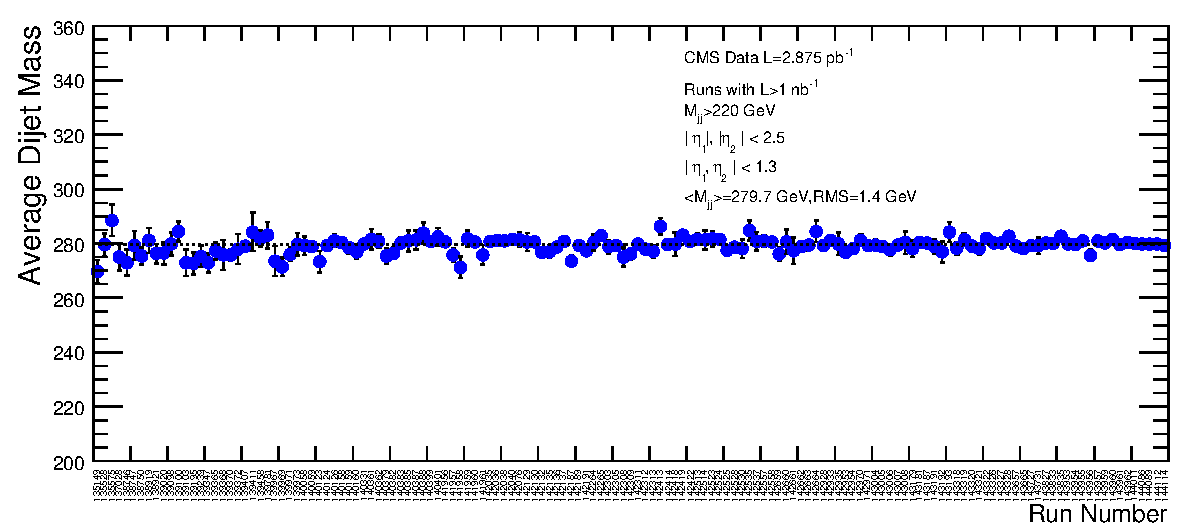
\includegraphics[width=0.9\textwidth]{Figures/MassVsRunNo.pdf} 
%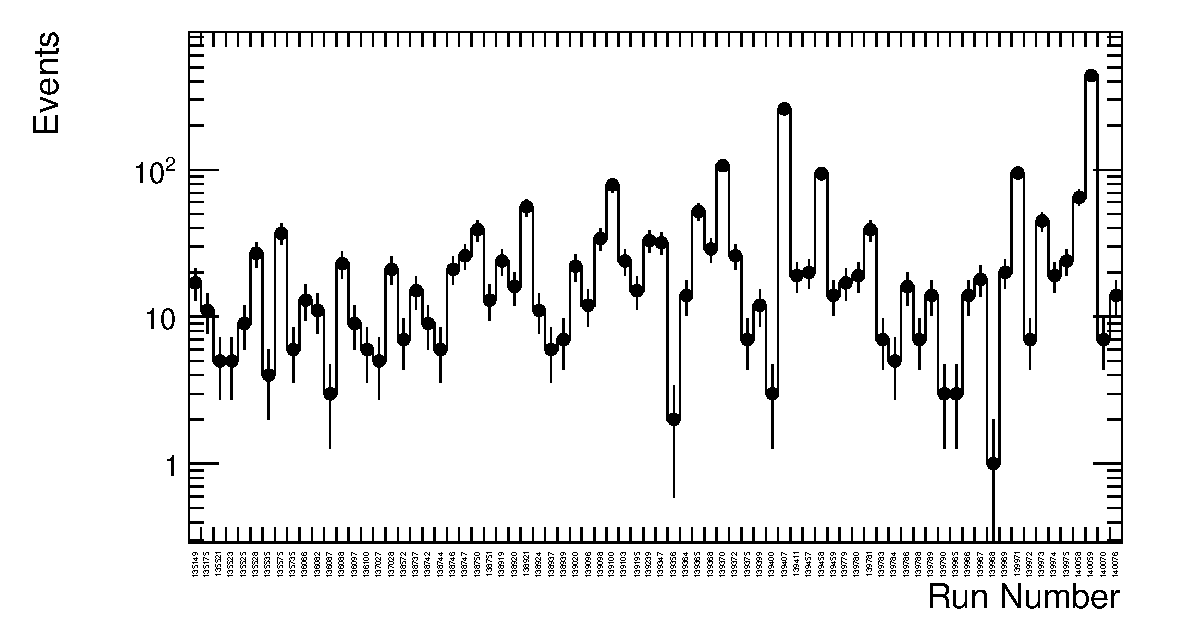
\includegraphics[width=0.9\textwidth]{Figures/Events.pdf}
\caption{Mean dijet mass vs run for runs with integrated luminosity greater than $1 nb^{-1}$ .}
    \label{MassVsRun}
  \end{center}
\end{figure}

\begin{figure}[!ht]
  \begin{center}
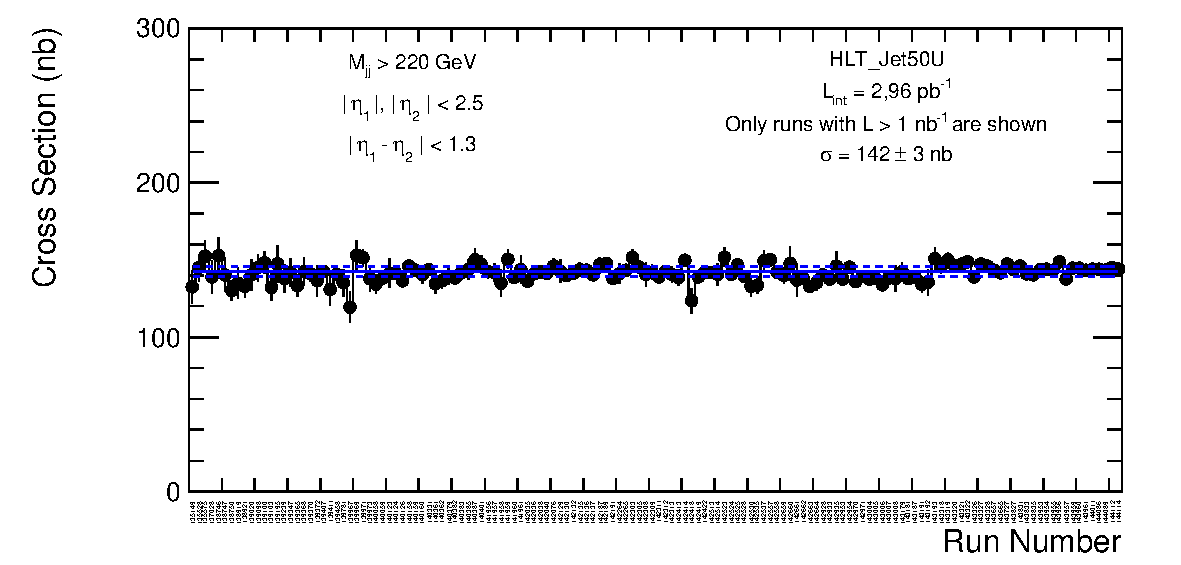
\includegraphics[width=0.90\textwidth]{Figures/XsecVsRunNo.pdf}
\caption{Number of dijet events passing the full selections, divided by the integrated luminosity of each run, vs. run.
Only runs with integrated luminosity greater than 1 $nb^{-1}$ passing the analysis selection are shown.}
    \label{XsecVsRun}
  \end{center}
\end{figure}

\begin{figure}[!ht]
  \begin{center}
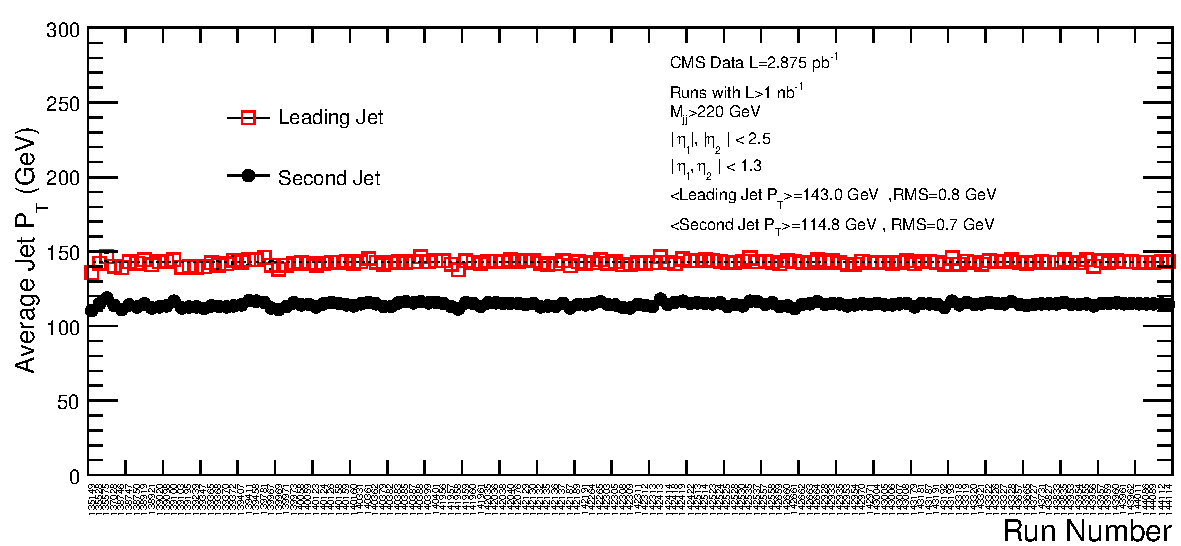
\includegraphics[width=0.49\textwidth]{Figures/PtVsRunNo.pdf}
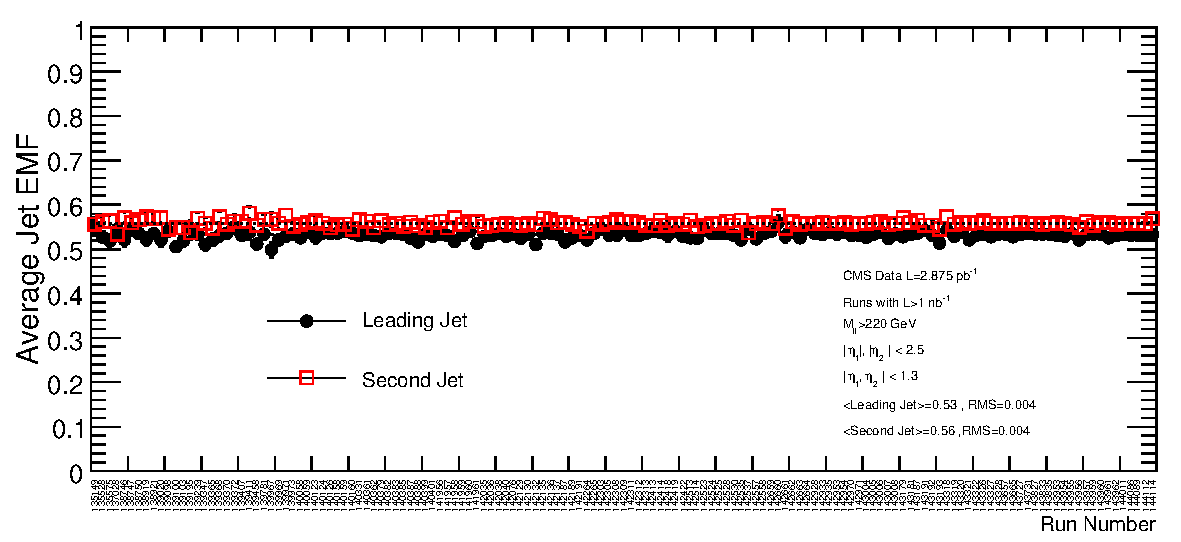
\includegraphics[width=0.49\textwidth]{Figures/EmfVsRunNo.pdf}
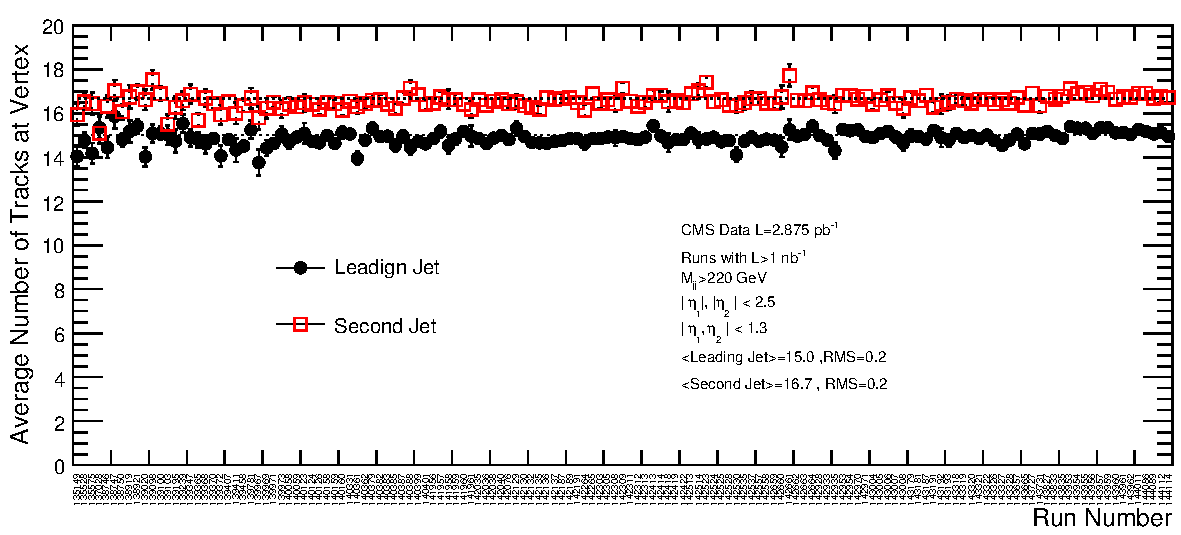
\includegraphics[width=0.49\textwidth]{Figures/NtrkVtxVsRunNo.pdf}
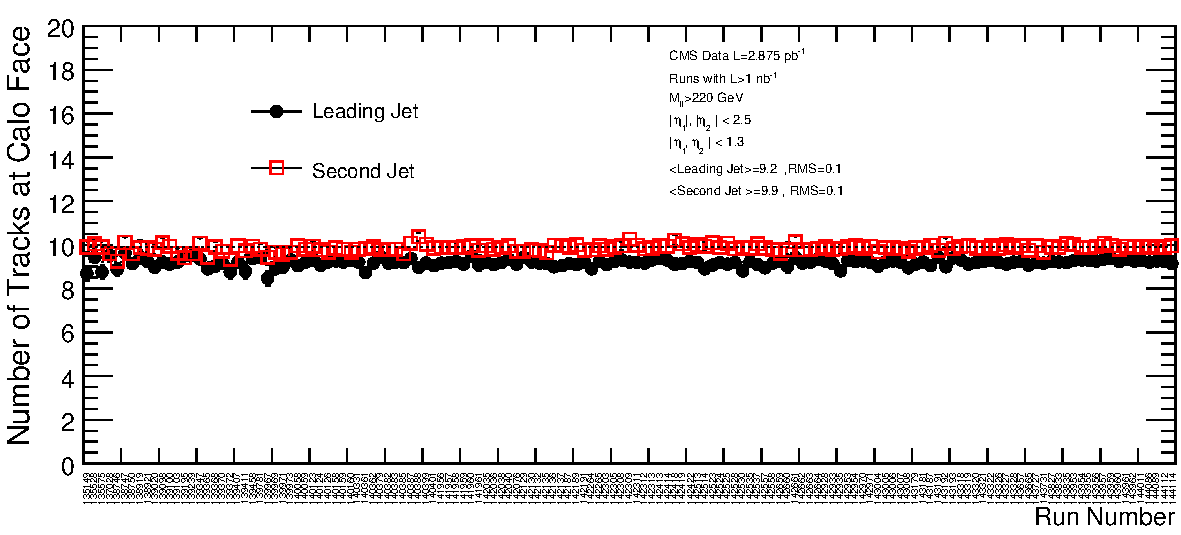
\includegraphics[width=0.49\textwidth]{Figures/NtrkCaloVsRunNo.pdf}
\caption{Mean value of jet properties for the leading jet (solid circles) and the second jet (open squares) vs. run: 
\pt (Top-Left), EMF (Top-Right), number of tracks associated with the jets at the vertex (Bottom-Left), number of tracks associated with the jets at the calorimater face (Bottom-Right). Only runs with integrated luminosity greater than $1 nb^{-1}$ are shown.}
    \label{JetPropertiesVsRun}
  \end{center}
\end{figure}

\clearpage
\subsubsection{Spectrum and QCD}
The measured dijet mass spectrum is shown in Fig~\ref{Spectrum}. The mass spectrum
is defined by 

\begin{equation}
\frac{d\sigma}{dm} = \frac{1}{\int Ldt} \frac{N_{i}}{\Delta m_i}
\label{eqXsec}
\end{equation}
where $m$ is the dijet mass, $N_i$ is the number of events in the $i$-th dijet mass bin, and $\Delta m_i$ is the width of the $i$-th 
dijet mass bin, and the integrated luminosity is $\int Ldt$.
This data is also tabulated in Appendix~\ref{appData}.  The bin width is approximately the dijet mass 
resolution, and gradually increases as a function of mass.
The data is compared to a QCD prediction from the PYTHIA MC and the full CMS simulation.
The normalization of the prediction is absolute, it has not been normalized to
the data in this plot.
Also shown in Fig~\ref{Spectrum} is the senstivity of the QCD + CMS simulation 
to a 10\% systematic uncertainty in the jet energy discussed in section~\ref{JESerror}.
The vertical error bars on the data are Poisson uncertainties, the horizontal
bars are the bin widths. Bins with zero events are indicated by a Poisson vertical error bar 
extending up to 1.8 events.
In Fig.~\ref{DataOverPythia} we show the ratio of 
the data to the PYTHIA prediction, which demonstrates at a fine scale the level of
agreement between data and PYTHIA. We can see that the 10\% uncertainty in the JES corresponds
to roughly a factor of 2 uncertainty in the observed cross section.
The PYTHIA QCD MC prediction is in good agreement with the data.   The highest mass dijet
event is at 2.05 TeV. 

%This can be seen from summation of the differential plot Fig~\ref{Spectrum} to 
%give the integral plot from the lower bin edge to infinity in Fig~\ref{Integral}. Conservatively,
%we expected 1 event above 1.4 TeV, and we observed 1 event above 1.4 TeV, and it happened to 
%occur at 2.13 TeV.  More aggressively, we expected 0.05 events above 2.1 TeV and we observed 
%1 event, which has a Poisson probability of 5\% which is still only about a 2 $\sigma$ effect.



\begin{figure}[!ht]
  \begin{center}
   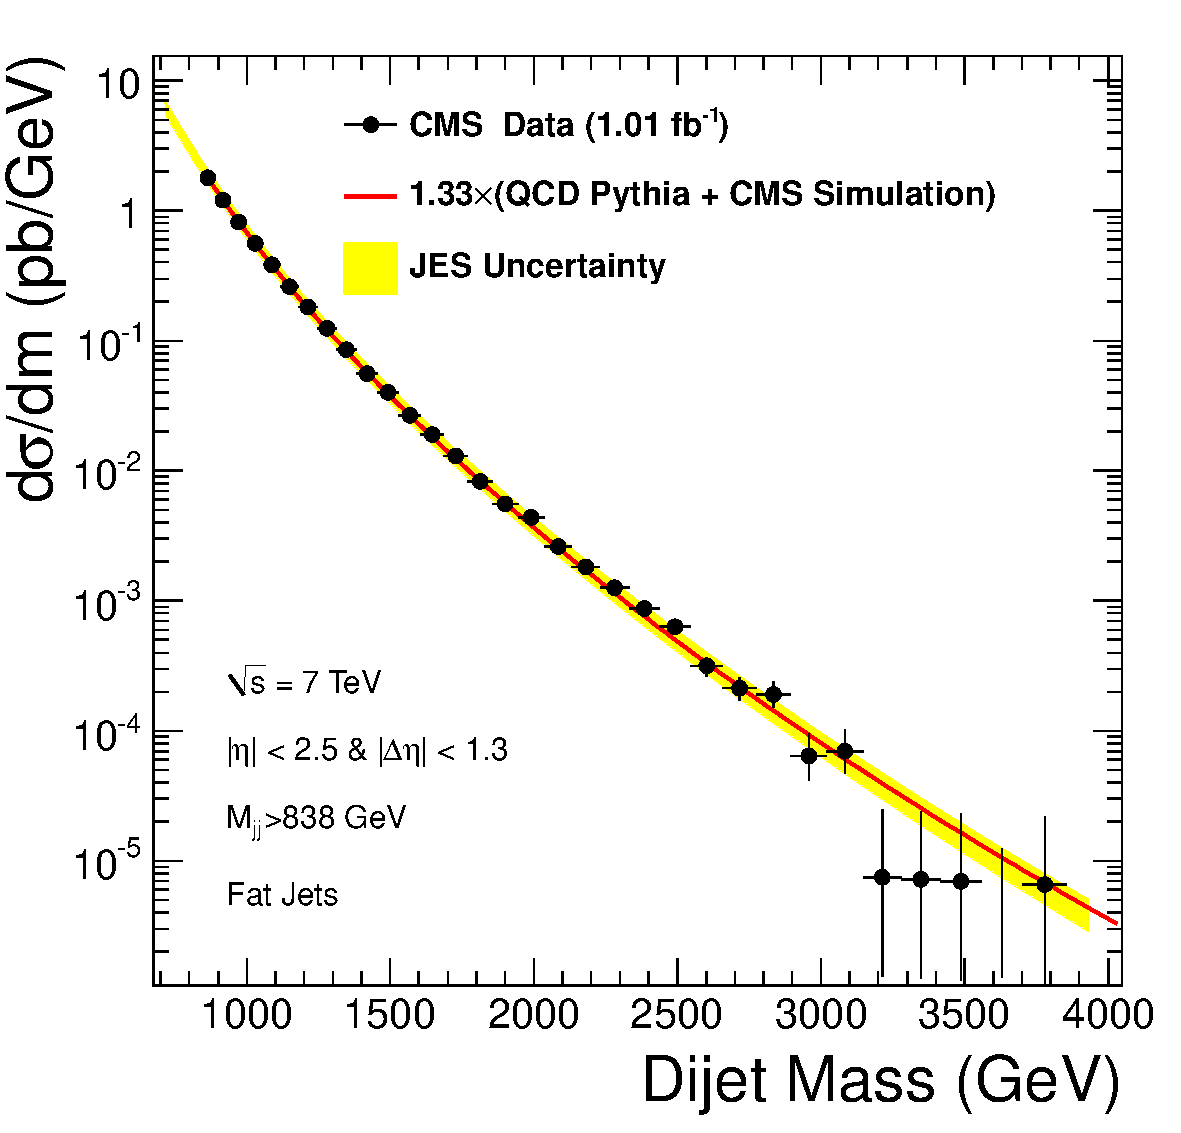
\includegraphics[width=\textwidth]{Figures/dijet_mass_Xsec.pdf}
    \caption{ The dijet mass spectrum data (points) is compared to a QCD MC prediction (histogram). Both the
    data and QCD prediction are absolutely normalized using the integrated luminosity.
    The band shows the sensitivity to a 10\% systematic uncertainty on the jet energy scale.}
    \label{Spectrum}
  \end{center}
\end{figure}

\begin{figure}[!ht]
  \begin{center}
   \includegraphics[width=\textwidth]{Figures/data_over_pythia.pdf}
    \caption{ Ratio of the dijet mass spectrum divided by the QCD Pythia prediction. Both the
    data and QCD prediction are absolutely normalized using the integrated luminosity.
    The band shows the sensitivity to a 10\% systematic uncertainty on the jet energy scale.}
    \label{DataOverPythia}
  \end{center}
\end{figure}

%\begin{figure}[!ht]
%  \begin{center}
%   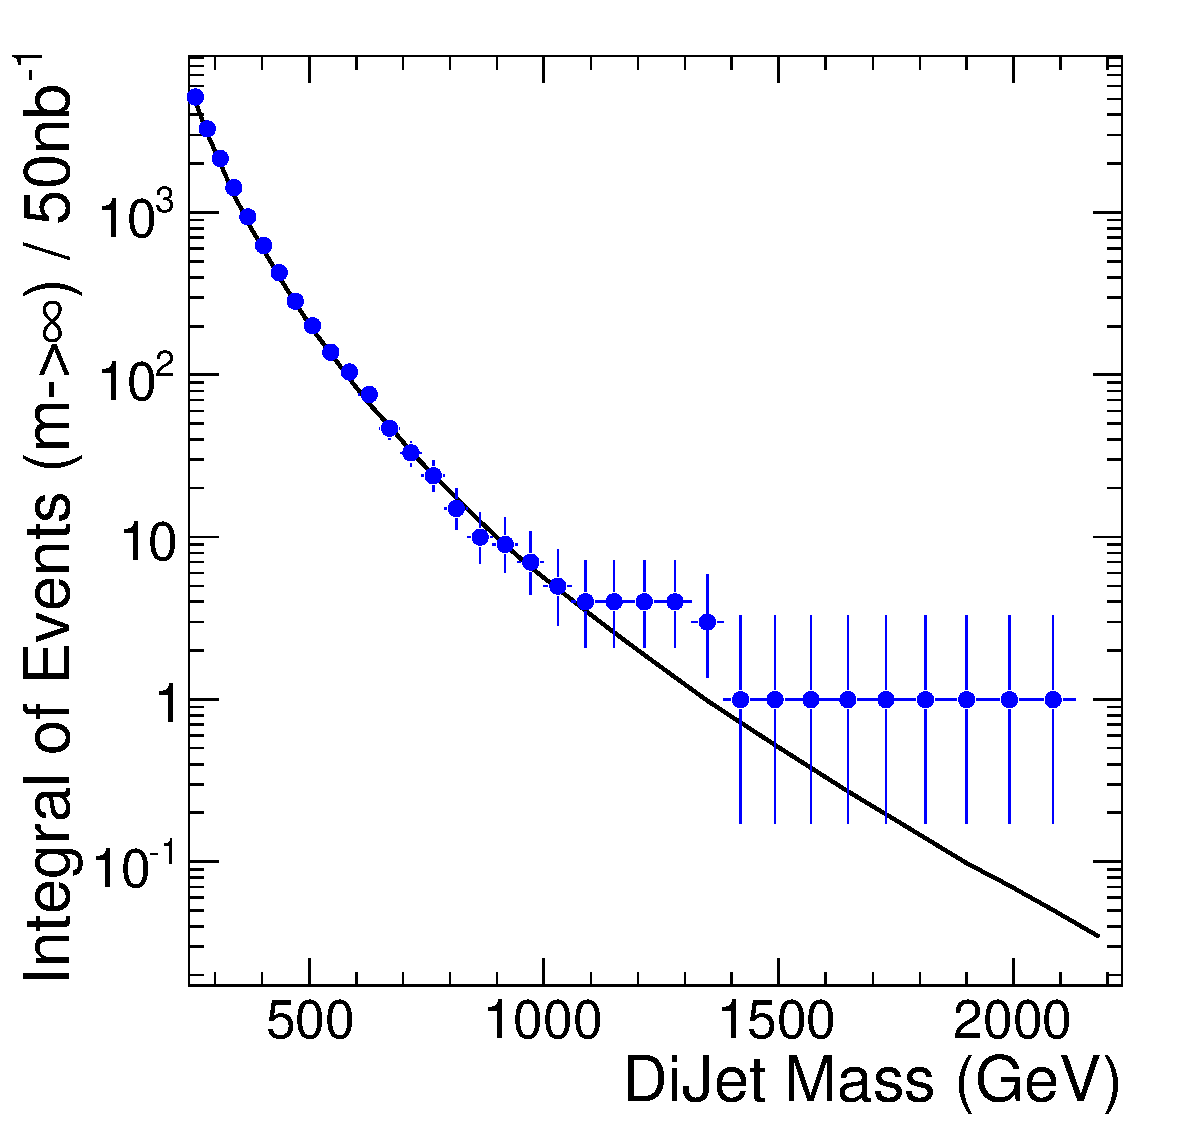
\includegraphics[width=\textwidth]{Figures/EventIntegral.pdf}
%    \caption{ The integrated event rate above a dijet mass threshold for the data (points) and 
%    the PYTHIA QCD prediction (curve).  The thresholds correspond to the lower edge of the mass bins
%    used in Fig.~\ref{Spectrum} and \ref{DataOverPythia}. The statistical errors on the points are 
%    highly correlated, because each point contains all the other points with higher dijet mass threshold.}
%    \label{Integral}
%  \end{center}
%\end{figure}

\clearpage

\subsection{Systematic Uncertainty on Jet Energy Scale}
\label{JESerror}
The jet energy systematic uncertainty band shown in Fig.~\ref{Spectrum} comes
from the JetMET guideline uncertainty of 10\% in the jet energy scale.
It is, by far, the dominant uncertainty in the measurement of the dijet
mass spectrum, and is also one of the largest uncertainties in the new particle
search.  The jet energy uncertainty at CMS is currently being explored with
in situ measurments which will ultimately provide a measure 
of the actual uncertainty~\cite{PAS_JME_07-002}.


As of today we can already see 
from measurements of photon plus jet balance~\cite{PAS_JME_10-003, CMS_AN_2010/141}
that the jet energy scale in the MC may very well be better than the 10\% currently being assigned. 
The jet response measured with photon + jet balance in the data, 
is in good agreement with the same response measured with the MC~\cite{PAS_JME_10-003} and constrain 
any difference to be well within the quoted 10\%. Due to the low statistics and
poorly understood calibration systematics and this early stage of the calibration analysis, JetMET
is not quoting an error yet based on this data, but JetMET is confident that the data do
indicate that 10\% is safe. 


At an even more fundamental level, we already see from
measurements of single particle response~\cite{PAS_JME_10-008, CMS_AN_2010/179}, that
the barrel calorimeter is responding as expected to input charged particles to better than 3\%.
Since a jet is made up of particles the uncertainty in the jet response can be 
constrained by the uncertainty in the constituent particle response.  The most uncertain
component is the charged pion response, as neutral pions are the other dominant contributor and they have well
understood response in the barrel ECAL.  The response of the ECAL plus HCAL to isolated 
charged particles measured in the barrel shows excellent agreement between
data and MC. Further, the MC simulation was tuned on test beam measurements of charged pions over
a wide range of momentum, and the tuning was quoted to be good to within 3\%.  Given these facts,
it is highly unlikely that the jet energy scale could be off by more than 10\% 
in the barrel.

We have also checked the energy scale of CaloJets against the energy scale
of particle flow jets in Figure~\ref{PFresp}.  Starting with the 
two leading PF jets in the event with $|\eta|<1.3$, we find the matching CaloJets that
are closest in $\Delta R$, plot the ratio of the corrected CaloJet to 
corrected PF jet $p_T$, and find the mean. The corrected CaloJet $p_T$ 
is in good agreement with the corrected PF jet $[_T$, well within 2\% at all 
$p_T$, demonstrating good agreement
between the jet energy scale defined by calorimetry alone and the jet energy
scale defined by tracking and calorimetry combined.
\begin{figure}[!ht]
  \begin{center}
   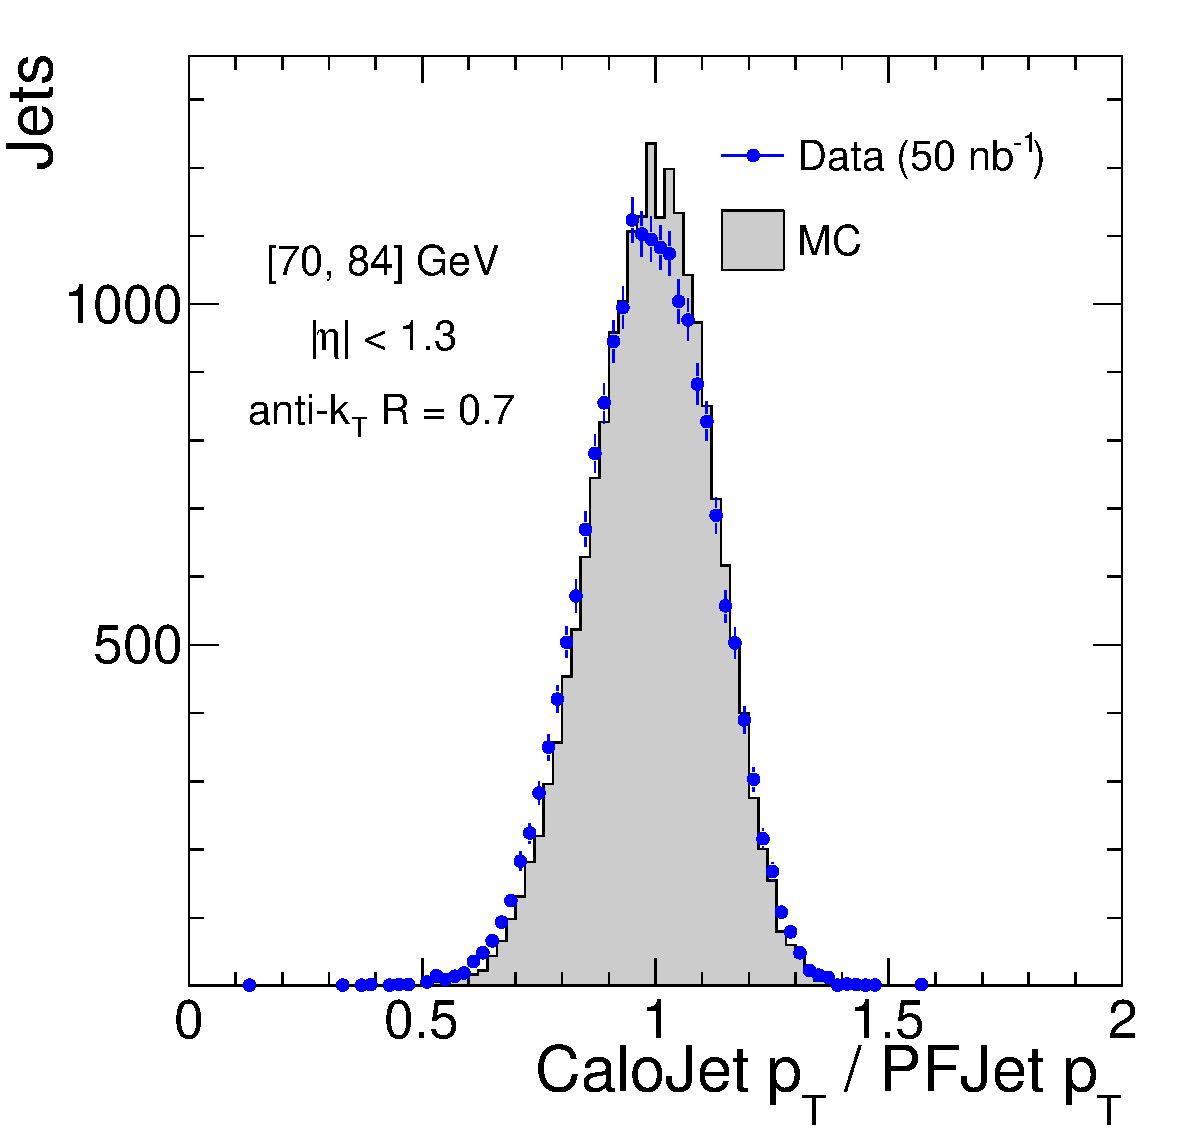
\includegraphics[width=0.32\textwidth]{Figures/caloRsp_Pt70to84.pdf}
   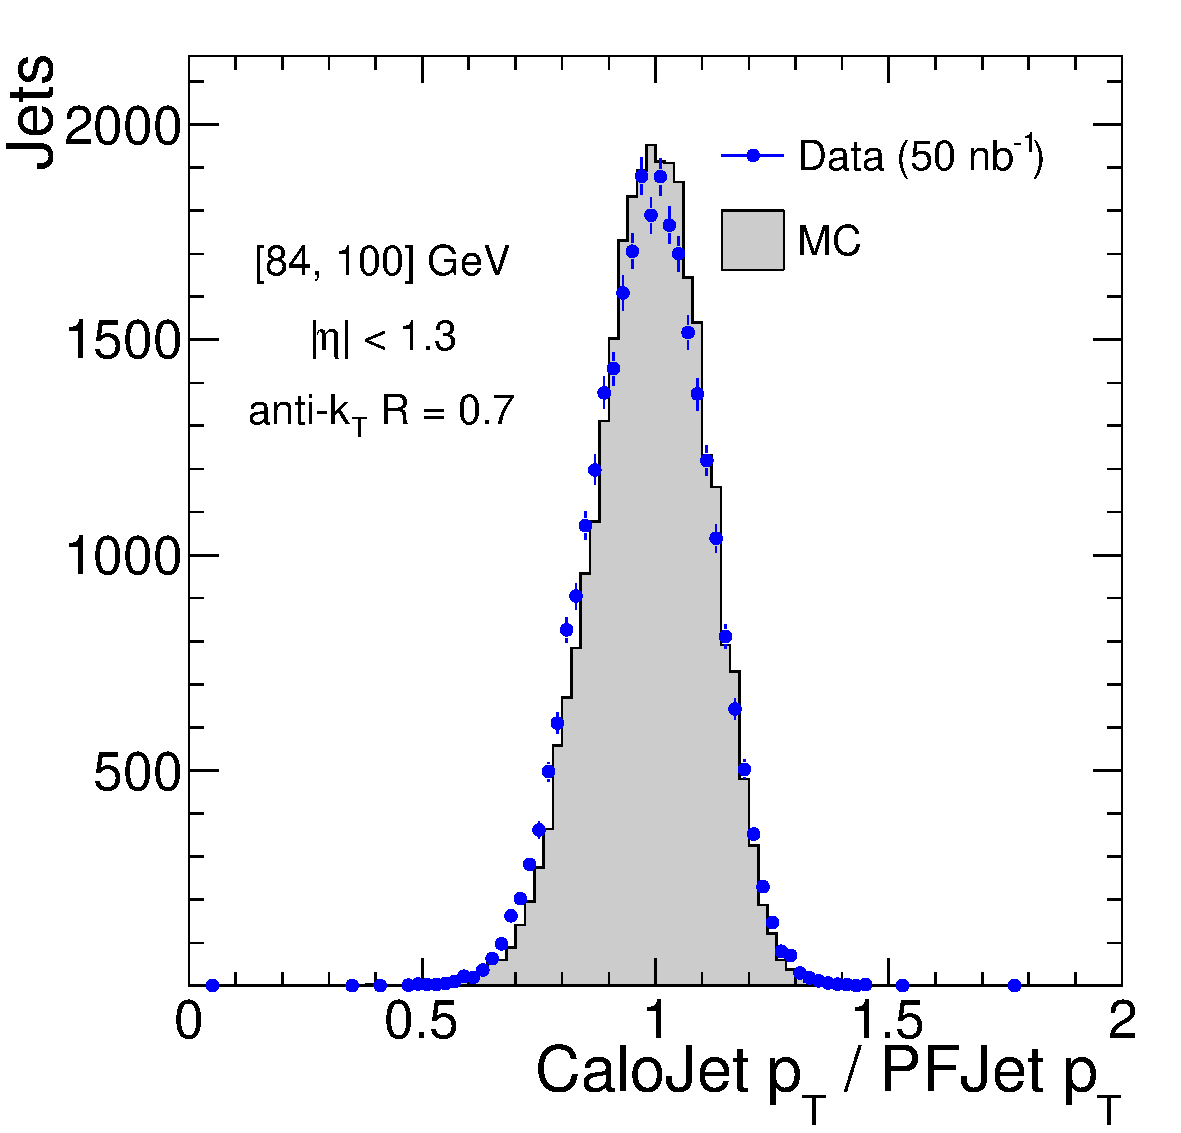
\includegraphics[width=0.32\textwidth]{Figures/caloRsp_Pt84to100.pdf}
   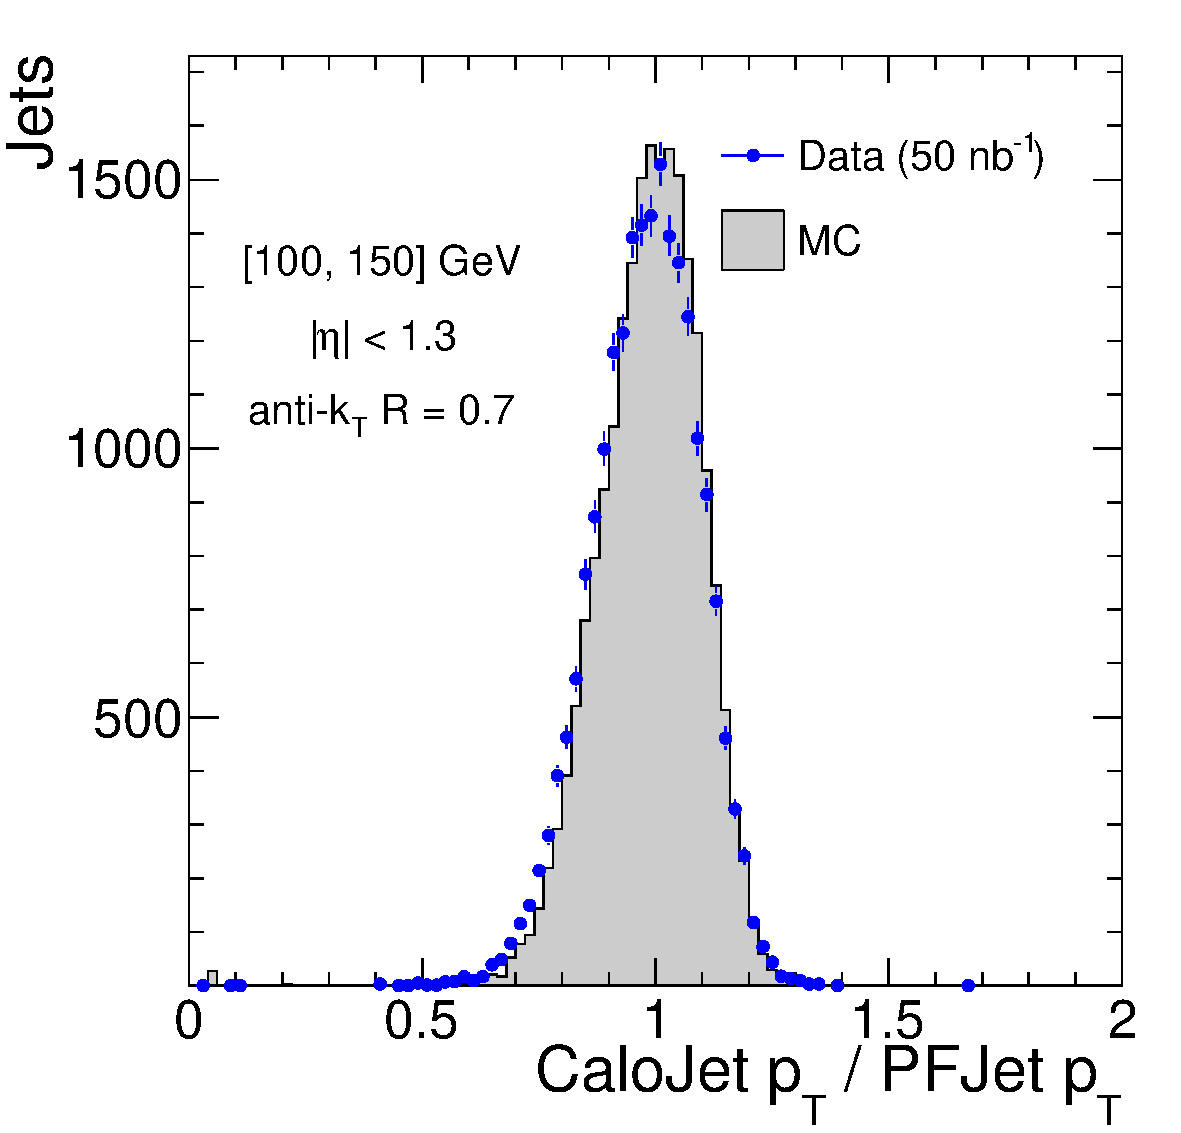
\includegraphics[width=0.32\textwidth]{Figures/caloRsp_Pt100to150.pdf}
   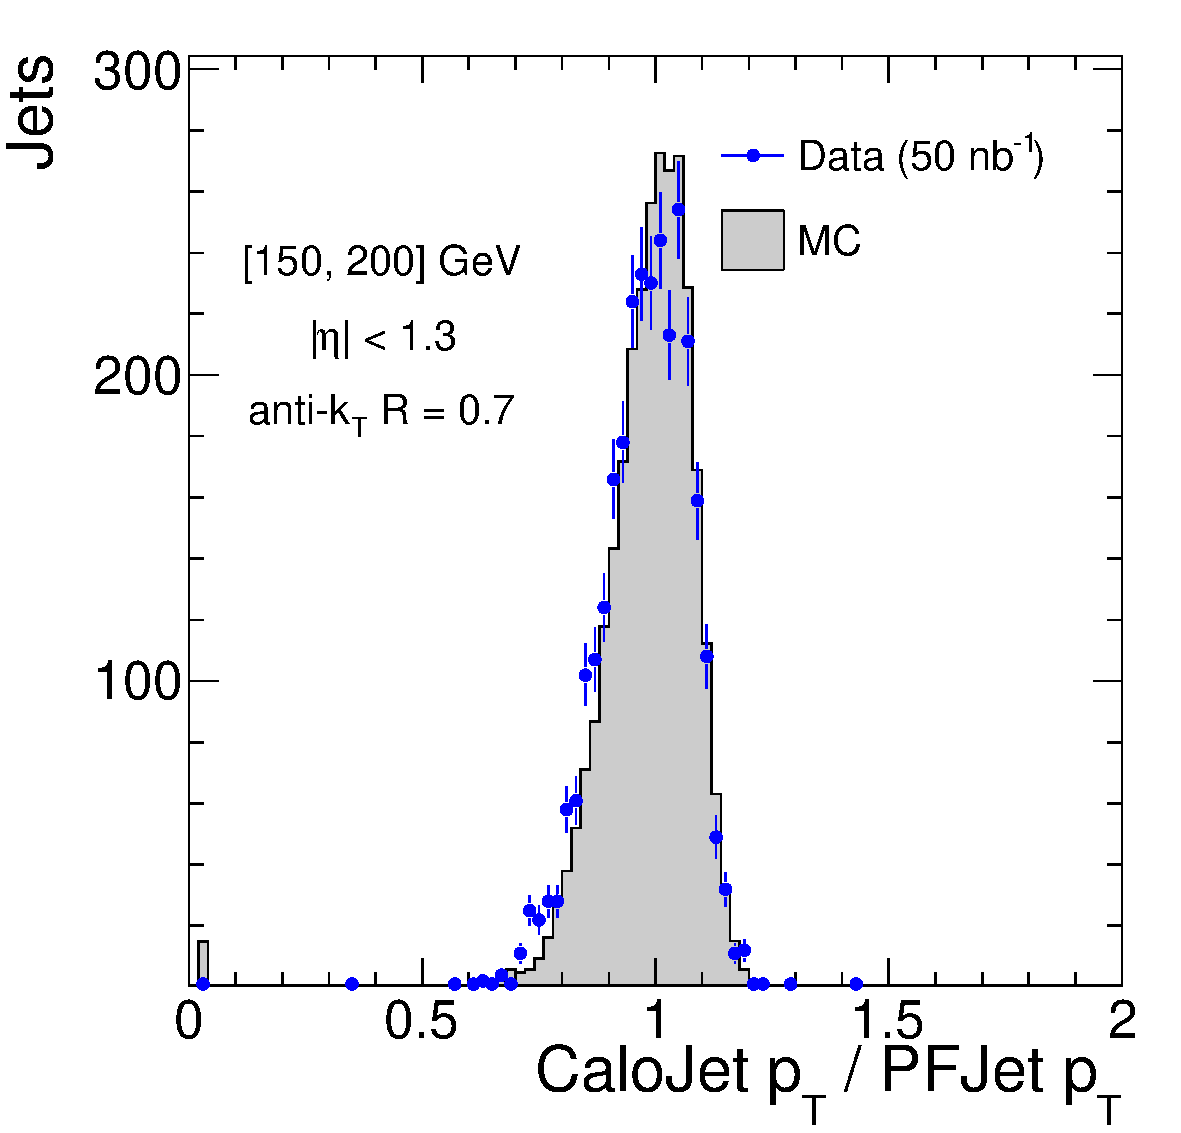
\includegraphics[width=0.32\textwidth]{Figures/caloRsp_Pt150to200.pdf}
   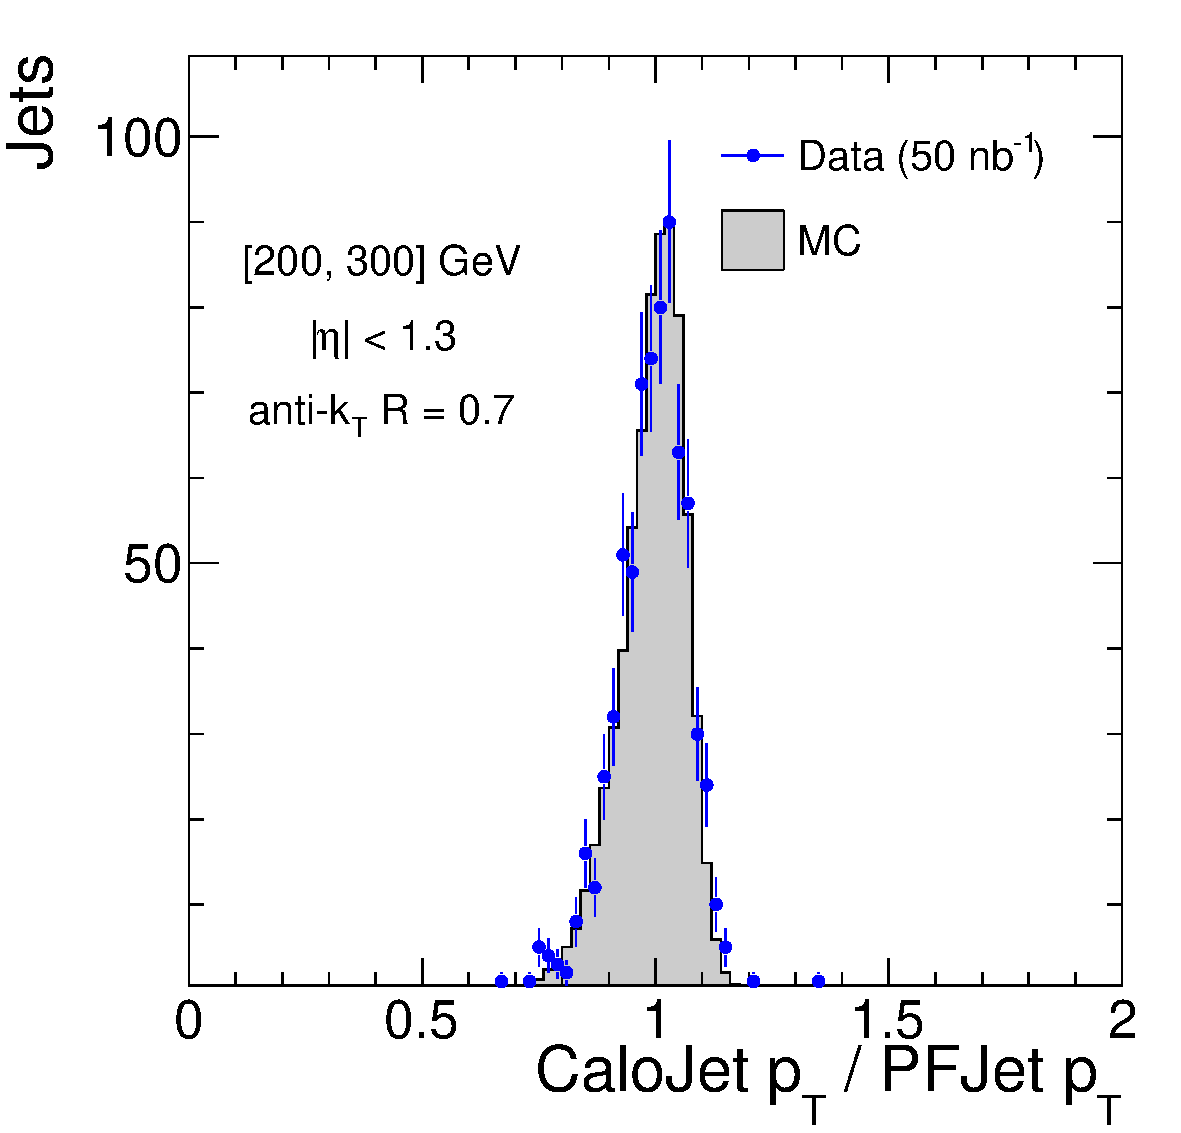
\includegraphics[width=0.32\textwidth]{Figures/caloRsp_Pt200to300.pdf}
   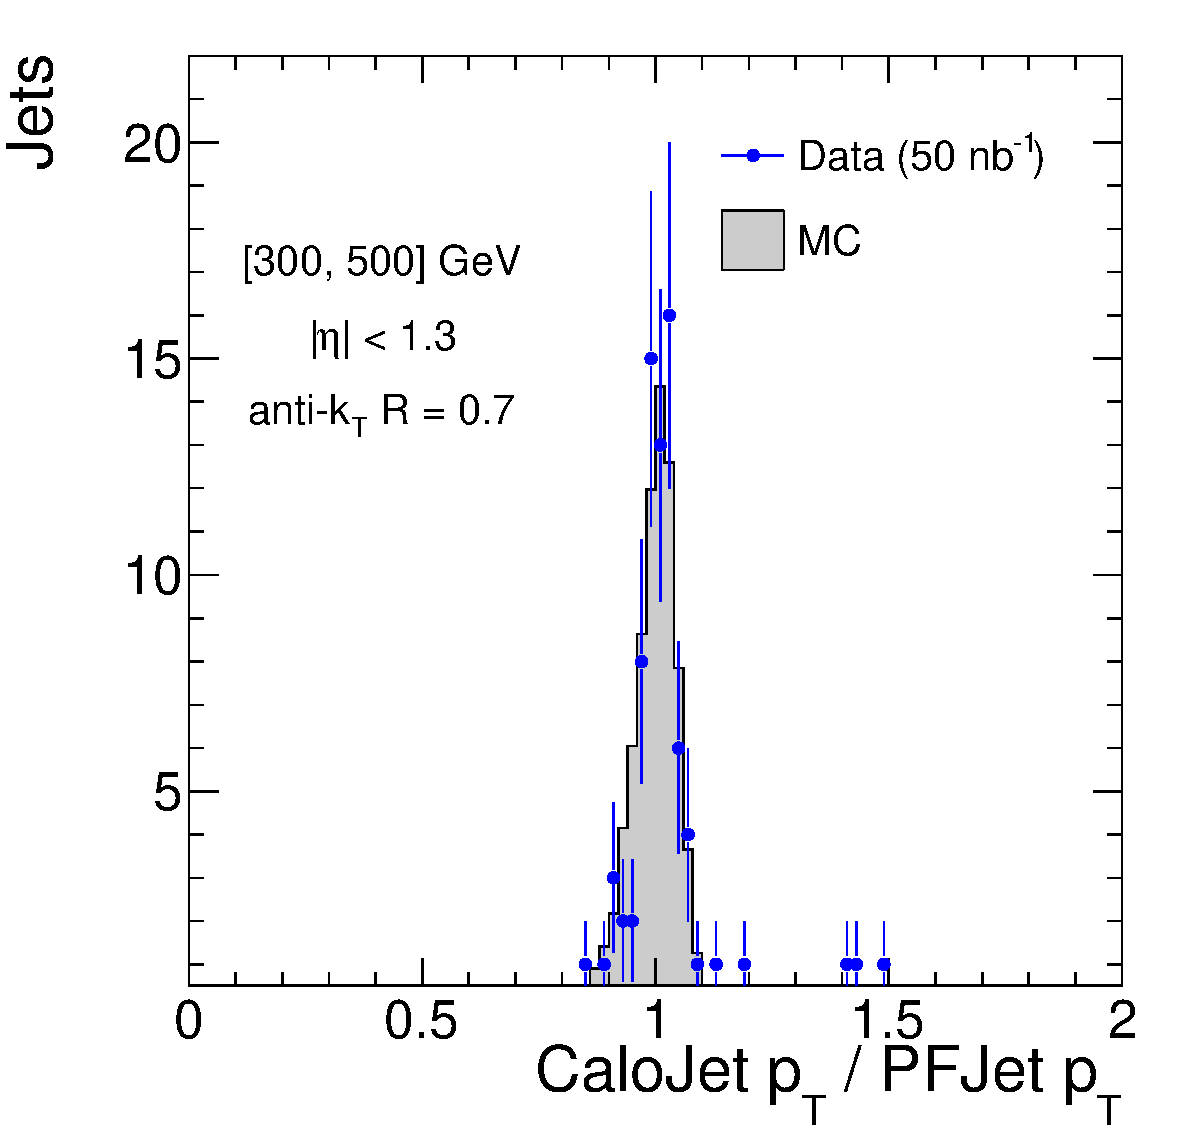
\includegraphics[width=0.32\textwidth]{Figures/caloRsp_Pt300to500.pdf}
   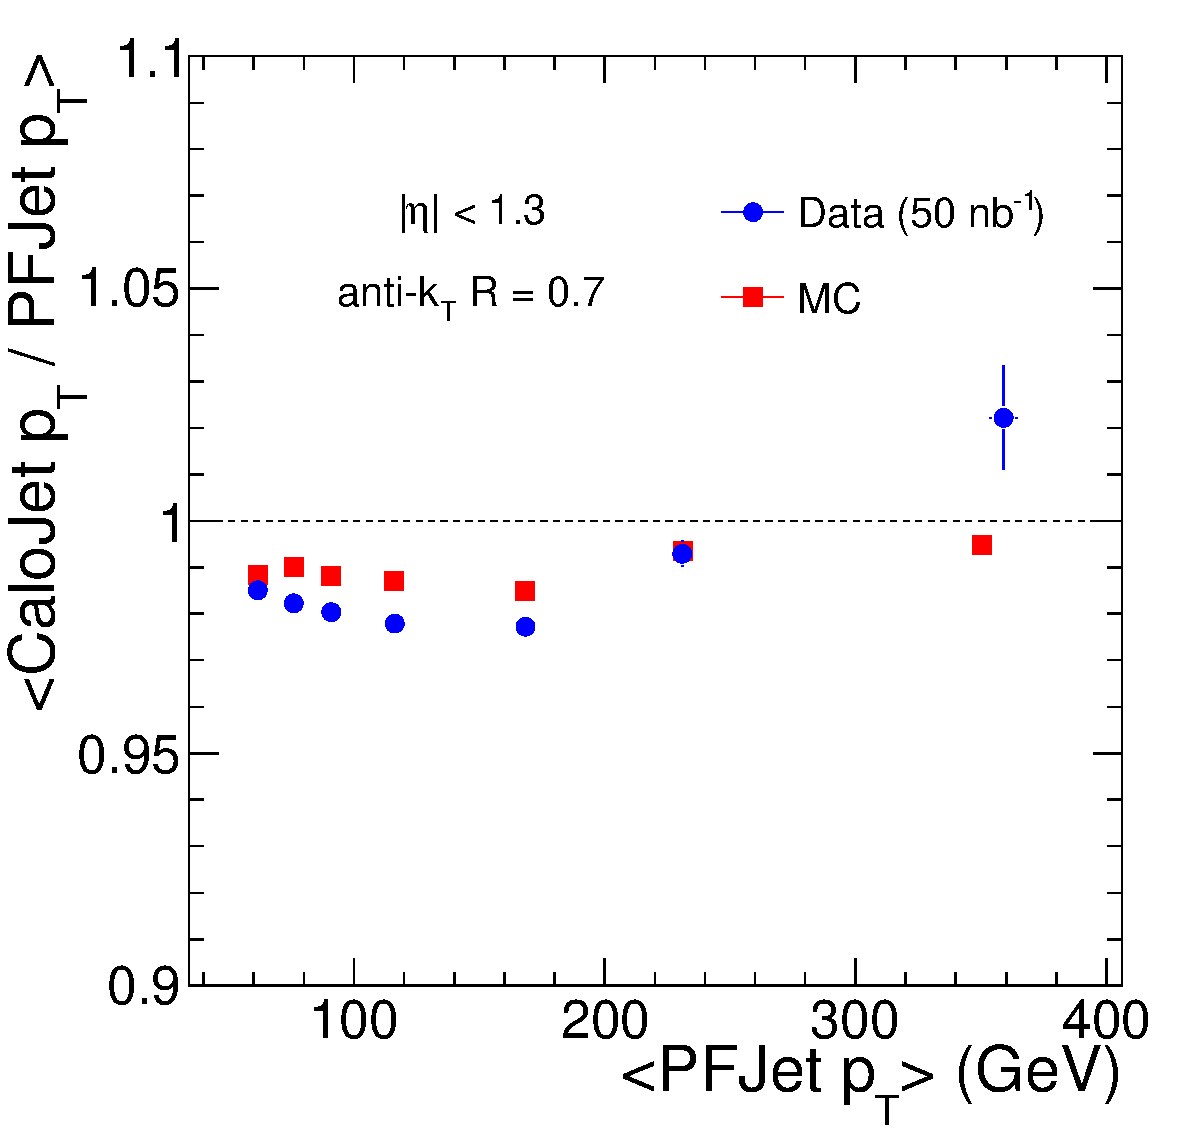
\includegraphics[width=0.8\textwidth]{Figures/PFvsCalo.pdf}   
    \caption{Distributions of Corrected CaloJet $p_T$ / Corrected PFJet $p_T$ 
    for leading jets which have $|\eta|<1.3$ 
    for six intervals of Corrected PF jet $p_T$ (top six plots) and the mean value of 
    this relative response as a function of the mean Corrected PF jet $p_T$ 
    (bottom plot).}
    \label{PFresp}
  \end{center}
\end{figure}

In situ data indicate that the 10\% guideline provided by JetMET on the jet energy scale uncertainty
is a conservative (safe) estimate.  

\subsection{Highest Mass Dijet Events}

Event displays of the ten highest mass dijet events are shown in 
Appendix~\ref{appEvents}.  They all look like good events, with
collimated calorimeter energy deposits and associated tracks.  Table~\ref{table_highmass2} in the 
Appendix lists the basic properties of 
the calorimeter reconstrution for these events.  
The highest
dijet mass observed is at 1.92 TeV as already mentioned. 

%In Appendix~\ref{appEvents} in table~\ref{table_highmass3} we list the 
%$p_T$ and dijet mass for these events from particle flow reconstruction
%of the jets (PFjets), which employs tracking in addition to the calorimeter.
%The $p_T$ and dijet mass values are very similar.  Here the PFjets have been
%matched to the corresponding leading CaloJets and are shown in that order
%in table~\ref{table_highmass3}.

%In Fig.~\ref{PF}, we
%show the difference in corrected jet $p_T$ between the leading 
%CaloJets and particle flow jets.
%The mean difference is $\Delta p_T= -0.5$ GeV out of 
%about 300 GeV.  The RMS of the difference between CaloJets and
%PFJets is 15 GeV.  This is in good agreement with the expected RMS from the 
%MC of 18 GeV: this expected RMS takes into account significant correlations 
%between the two reconstruction techniques~\cite{refMikko}. The mean 
%difference of the dijet mass between the two techniques is $2\pm 10$ GeV, 
%and the RMS of the difference in dijet mass is 33 GeV, which makes sense compared
%to $p_T$, but we do not have 
%available an estimate of this RMS from MC that takes into account correlations.
%The good agreement
%between calorimeter and particle flow jet reconstruction techniques for 
%the 10 highest mass dijet events indicates that jet reconstruction with 
%tracking is confiriming our 
%calorimeter based reconstruction technique.


%\begin{figure}[!ht]
%  \begin{center}
%   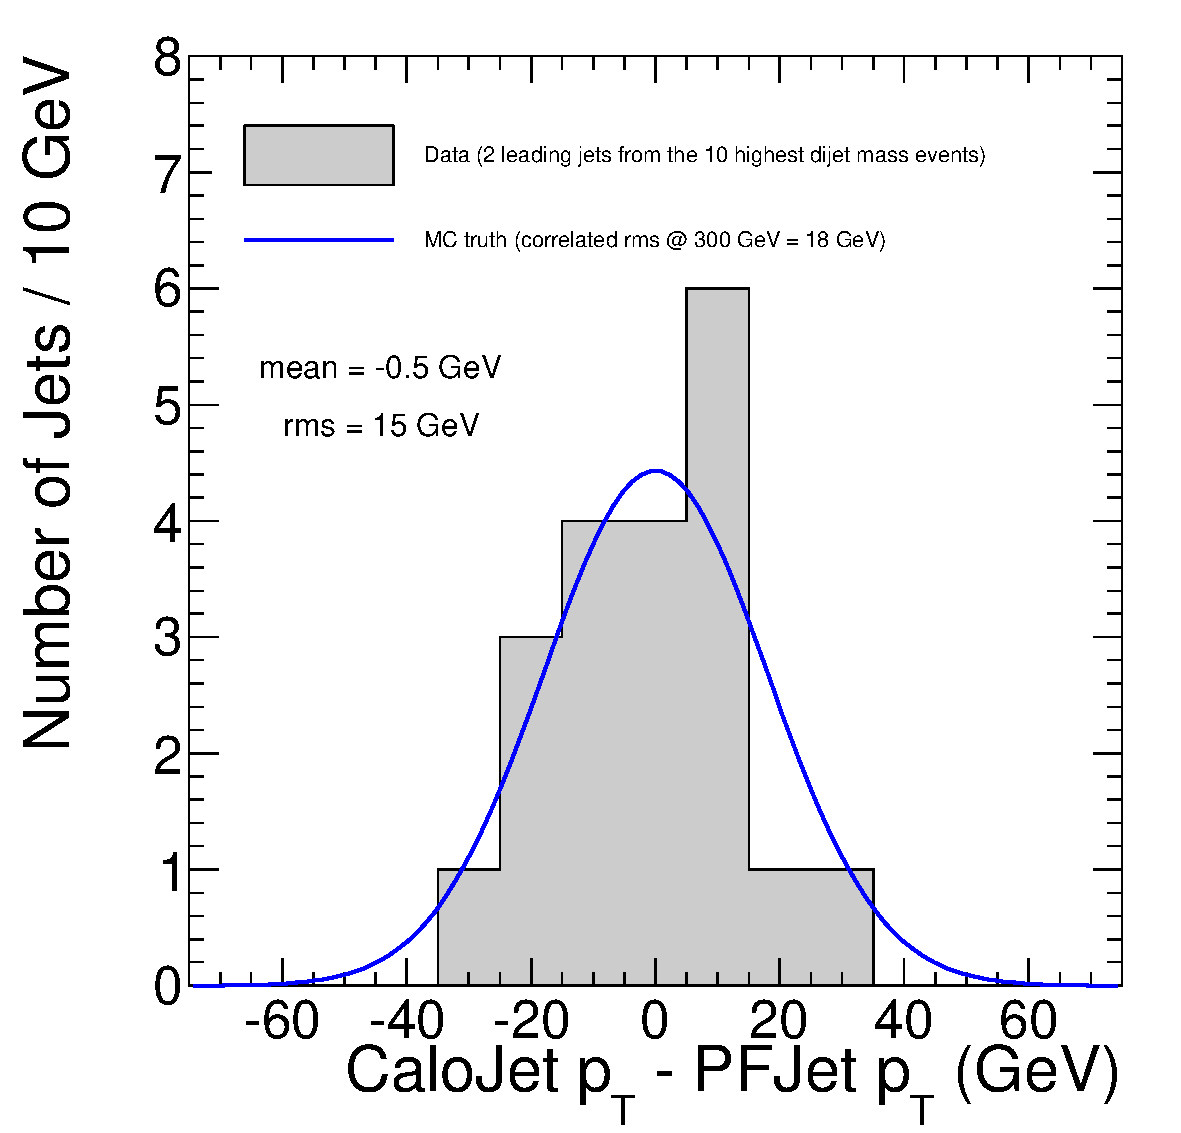
\includegraphics[width=0.7\textwidth]{Figures/CaloPFCorrelation.pdf}
%    \caption{The difference in corrected jet $p_T$ between the leading CaloJets
%    and the leading matched particle flow jets (histogram) for the 10 highest dijet
%    mass events is compared with an estimate of the expected difference from MC (curve)
%    taking into account correlations. }
%    \label{PF}
%  \end{center}
%\end{figure}
\clearpage

\subsection{Dijet Mass Spectrum and Fit}


\begin{figure}[!ht]
  \begin{center}
   \includegraphics[width=\textwidth]{Figures/DijetMass_withFit.pdf}
    \caption{The dijet mass distribution (points) compared to a smooth background fit (solid
curve). }
    \label{Fit}
  \end{center}
\end{figure}


Fig.~\ref{Fit} shows the dijet mass spectrum from Fig.~\ref{Spectrum} compared to
a fit. Here we model the background to a dijet resonance coming from standard model dijet production
using a simple parameterization. Our first test for whether there is a bump or other local
effect in the data is to simply see if we can get a good fit to a smooth parameterization.
Fig.~\ref{Fit} also shows the parameterization fitted to the data. We get a $\chi^2$ of 32.3 
for 31 degrees of freedom for the fit.  The parameterization chosen is~\cite{Aaltonen:2008dn,ATLAS_Search} 


\begin{equation}
\frac{{\rm d}\sigma}{{\rm d}m} = 
\frac{P_{0} (1 - m/\sqrt{s})^{P_{1}}}{(m/\sqrt{s})^{P_{2} + P_{3} ln
(m/\sqrt{s})}}
\label{eqParam}
\end{equation}

Fig~\ref{FracDiff} shows the fractional differences between data and the fit function, (data-fit)/fit, which show no significant evidence 
of a peaks above the background fit. The most significant upward fluctuation observed is studied in section~\ref{significance}. 
In the fractional difference plot the error bars are in units of the fit in the bin.
Fig.~\ref{FracDiff} show the pulls, defined as \textit {(Data-Fit)/Error}, which are consistent with statistical fluctuations and 
are oscillating around zero. In the pulls plot the error bars are always exactly 1, because they are in units of the error in the bin.

\begin{figure}[!ht]
  \begin{center}
        \includegraphics[width=0.9\textwidth]{Figures/Fractional_Diff.pdf}
    \includegraphics[width=0.9\textwidth]{Figures/Pulls.pdf}
    \caption{ \textit{Top})
The fractional difference between the dijet mass distribution (points) and a smooth
background fit as a function of dijet mass. \textit{Bottom}) The pulls distribution (Data-Fit)/Error as a function of dijet mass.}
    \label{FracDiff}
  \end{center}
\end{figure}
\clearpage
%%%%%%%%%%%%%%%
\subsubsection{Fit to Dijet Mass Spectrum with Various Parameterizations}
\label{sectionParam}

 
In Fig.~\ref{dijetmassFitParams} we show the dijet mass distribution,
$d\sigma/dm$, fit with three different parameterizations:  our default 4 parameter
fit and two alternate fits.
%%%%%%%%%%%%%%%%%%%%
\begin{figure}[!ht]
  \begin{center}
        \includegraphics[width=\textwidth]
                        {Figures/DijetMass_withFit_All.pdf}
    \caption{ 
The dijet mass data (points) is compared to fits (curves)
using our default fit function and three alternate fit functions.}
    \label{dijetmassFitParams}
  \end{center}
\end{figure}

\clearpage
The parameterizations are listed in equation~\ref{eqVariousParams}.

%%%%
\begin{eqnarray}
{\frac{d\sigma}{dm}} 
 &=& {\frac{P_{0} \cdot (1 - m/\sqrt{s})^{p_{1}}}{(m/\sqrt{s})^{p_{2} + p_{3} ln(m/\sqrt{s})}}} \, \, \, \mbox{(Default Fitwith 4-parameters)}. \cr
 & & \cr
 &=& {\frac{P_{0} \cdot {\Big(1-m/\sqrt{s}+P_3\cdot(m/\sqrt{s})^2\Big)^{P_1}}}{m^{P_{2}}}} \, \, \,\mbox{ (Alternate Fit A with 4-parameters)}. \cr
 & & \cr
 &=& {\frac{P_{0} \cdot {(1-m/\sqrt{s}\,)^{P_1}} }{m^{P_{2}}}}, \, \, \, \mbox{(Alternate Fit B with 3-parameters)} \cr
\label{eqVariousParams}
\end{eqnarray}
%%%%


The default four parameter function was used by CDF in run II~\cite{Aaltonen:2008dn} and is used 
by ATLAS~\cite{ATLAS_Search}. It gives a good fit with $\chi^2/DF=32.3/31$.
We have also explored two alternate parameterizations.  All parameterizations have a power law in them, because without
a power law we cannot get a good fit with only 3 or 4 parameters. 

Alternated fit B is a three parameter fit that was used by CDF in run IA~\cite{Abe:1995jz} and has the simplest QCD motivation,
althought all the parameterizations are motivated in a similar fashion.  It was used in much earlier versions of this CMS analysis
with significantly less luminosity.
It has a term in the numerator motivated by the parton distribution fall off
with fractional momentum, the same term as in the numerator of our default fit.
It includes a power law fall off with mass in the denominator, 
motivated by the QCD matrix element. The goodness of fit, $\chi^2/DF=39.3/32$, is significantly
worse than our default four parameter fit.

Alternate fit A is a 4-parameter function that was used by CDF 
in run IB~\cite{Abe:1997hm} and in the last version of this CMS analysis.
It similar to alternate fit B, except it has an additional term in the numerator to give flexibility beyond the
3-parameter fit. The goodness of fit, $\chi^2/DF=38.6/31$, is significantly worse than 
our default four parameter fit. Since this parameterization has the same number of 
parameters as our default fit, we use it to evaluate systematics on the background
functional form, and it should be conservative given the difference in $\chi^2$ between the
two fits.

Figure~\ref{dijetmassFits} shows the fractional 
differences between data and the fit function, (data-fit)/fit, 
and the pulls, (data-fit)/error, for all three fits.

%%
\begin{figure}[!ht]
  \begin{center}
        \includegraphics[width=\textwidth]{Figures/Fractional_Diff_All}
        \includegraphics[width=\textwidth]{Figures/Pulls_All}
    \caption{ Top) Fractional difference (points) between the dijet mass distribution 
data and four fits as a function of dijet mass.
Bottom) Pulls for the data (points) compared to four fits as a function of dijet mass.}
    \label{dijetmassFits}
  \end{center}
\end{figure}

%\begin{figure}[!ht]
%  \begin{center}
%        \includegraphics[width=0.8\textwidth]
%                        {Figures/dijet_mass_Fit_FracDiff_23params.pdf}
%    \caption{
%    Fractional difference between the dijet mass distribution 
%data points and the 2-parameter fit (left) and the 3 and 4 parameter fits (right).}
%    \label{dijetmassFractionalDiffFit23params}
%  \end{center}
%\end{figure}
%%%%%%%%%%%%%%%%%%%%

\clearpage
